\chapter{Introdução}

\section{Por que cidades existem?}

Para Bauman, cidades são lugares de oportunidades e são movidas por ``newcomers'', pessoas que não são originalmente do lugar e são estranhos à sua realidade. Quando essas pessoas chegam nas cidades, elas apresentam novas perspectivas sobre problemas antigos e suas formas de pensar geralmente conflitam com tranquilidade consequente da familiaridade e convivência dos residentes bem estabelecidos. Apesar disso poder gerar incômodo aos nativos, é para o bem deles e da cidade que suas formas de ser sejam questionadas e desafiadas pelos estranhos. Para o autor, esse estado de inquietude e permanente sentimento de ``ser estrangeiro'' é o que leva as pessoas e a cidade a buscar reflexão, debate e inovação \cite{bauman2003city}.

Para Jane Jacobs, uma característica que determina o sucesso de uma cidade é sua vitalidade. A autora defendia que a vida na cidade depende fortemente das dinâmicas sociais, das interações cotidianas de seus residentes. Para Jacobs, a cidade proporciona interações nos espaços públicos -- onde a vida urbana efetivamente acontece -- e possibilita que as pessoas se conectem, encontrem, colaborem e prosperem juntas. Ela valorizava a diversidade, densidade e a mistura de usos do solo urbano, argumentando que a presença de uma variedade de estabelecimentos comerciais, residenciais e culturais em uma mesma área promove a interação entre diferentes grupos sociais e estimulava a criatividade e a inovação \cite{jacobs1961death}.

Do ponto de vista econômico, o triunfo da cidade se encontra nos benefícios de aglomeração e adensamento. Economias de aglomeração permitem que firmas diferentes escolham ficar geograficamente próximas umas das outras e encontrem benefício econômico ao reduzirem seus custos e aumentarem a produtividade. Jan Brueckner, em \textit{Lectures on Urban Economics}, delimita no capítulo 1 o racional econômico da existência de cidades, que se divide em quatro principais componentes.

A aglomeração tecnológica $(i)$ aumenta a produtividade dos trabalhadores, na medida em que os empregos são mais concentrados e há ``transbordamento'' de conhecimento entre as firmas da região. Além disso, uma oferta maior e mais diversa de trabalho, causa maior competitividade e eficiência na escolha da pessoa certa para cada cargo. Aglomerações pecuniárias $(ii)$ reduzem os custos das firmas, sem alterar sua produtividade. Com maior demanda por serviços como segurança, limpeza, contratação e advocacia, estes mercados se desenvolvem, tornam-se mais competitivos, eficientes e baratos. Inclusive, há serviços especializados de nicho, que podem estar disponíveis e acessíveis apenas em grandes centros urbanos. Aglomeração de varejo $(iii)$ traz ganhos para os consumidores e comerciantes. Quando o comércio está aglomerado, o consumidor pode escolher entre mais opções e se desloca menos entre seus destinos caso queria comprar mais de um item. Dessa forma, os consumidores ganham e os comerciantes também, visto que com mais consumidores e maior fluxo, maiores as vendas. Por fim, o custo de transporte $(iv)$ é um dos fatores que mais mudam quando há densidade. A redução do custo de transporte, que pode ser considerada uma economia de aglomeração pecuniária, acontece não apenas para os trabalhadores, que se deslocam menos às oportunidades de emprego, mas também às firmas que gastam menos transportando seus bens e serviços \cite{brueckner2011lectures}.

Dito isso, uma pergunta relevante é se as forças de aglomeração atuam sozinhas ou se precisam de incentivos e regulação. Caso o mercado por conta própria seja capaz de gerar o nível eficiente de aglomeração, a regulação geraria um peso morto. Entretanto, o mercado apresenta falhas, então a regulamentação pode ser importante para contrabalancear seus efeitos, ou até mesmo impedir que elas ocorram.

\section{Importância da regulamentação}
\label{sec:intro-regulacao}

Na literatura microeconômica há diversos modelos que tentam compreender as dinâmicas econômicas da cidade, analisando como as forças de mercado agem na ausência da regulação. Utilizando premissas formais e provas matemáticas, é possível resolver os modelos para algumas variáveis endógenas, como preço por metro quadrado na cidade, uso do solo, densidade populacional, entre outros. O que geralmente há de comum entre estes modelos, é que se o mercado receber um tratamento \textit{laissez-faire}, se observará um maior adensamento no centro, onde há oferta de emprego. Quando há múltiplos centros, ou pontos de transporte público de alta capacidade, também há maior adensamento no entorno deles \cite{papageorgiou2012essay, fujita1989urban,brueckner2011lectures}.

Entretanto, ao introduzir falhas de mercado nesses modelos, a organização da cidade na ausência de regulamentação pode estar associada cenários não desejáveis. Muitas vezes estas falhas de mercado encadeam uma expansão da mancha urbana, com implicações graves no meio ambiente, além da perda dos benefícios da aglomeração. Um exemplo de falha de mercado está relacionada ao tráfego de carros. Este meio individual diminui os custos de transporte para longas distâncias, possibilitando que os cidadãos habitem residências mais distantes de seus destinos. Todavia, além de causar uma expansão da mancha urbana, introduzir risco de acidentes e emitir poluentes, cada carro a mais que está na rua torna a viagem de todas as outras pessoas um pouco mais lenta. Apesar desses malefícios serem negligenciáveis nas escolhas individuais de utilizar ou não o carro, ou seja, um indivíduo racional não vai deixar de usar o carro, em uma cidade com milhões de habitantes, o custo individual negligenciado de cada carro se soma, de forma a ter um impacto significativo para a sociedade.

Nesse sentido, o governo poderia intervir, de forma a corrigir estas falhas de mercado, por exemplo, introduzindo um pedágio urbano. Dessa forma, seriam internalizadas as externalidades negativas dessa escolha individual de usar o carro. Com o dinheiro coletado desse imposto, poderiam ser compensados os danos causados, através de investimentos públicos. Entretanto, tal medida é difícil de ser implementada, levando os tomadores de decisão a tomar outro caminho no combate às externalidades. Regular os padrões construtivos, pode ser uma forma alternativa de lidar com o problema, impedindo que as externalidades aconteçam. Ao invés de cobrar um imposto pelo uso do automóvel, o plano diretor de São Paulo optou por limitar o número de vagas de garagem em empreendimentos em determinadas regiões, por exemplo \cite{PDE}.

Um instrumento regulatório utilizado em muitas grandes cidades é o Coeficiente de Aproveitamento (CA). Este será explicado em maior detalhe adiante, mas em linhas gerais, ele é capaz de definir a densidade construtiva da região. Ao criar limites mínimos e máximos de CA, os governos das cidades pretendem definir as localidades que recebem mais habitantes, como uma forma de combate às externalidades que o mercado \textit{laissez-faire} geram. Por exemplo, para garantir que os usuários de carro não habitem regiões mais distantes, é possível implementar um CA baixo nas periferias e aumentá-lo na medida em que se aproxima do centro. 

Caso o CA seja maior do que o mercado demanda, o CA observado será inferior ao limite, ou seja, a regulação não impacta essa região. Nas regiões em que a demanda por habitação é maior do que o permitido, os indivíduos vão ter que escolher outras regiões. Nesse sentido, caso a demanda reprimida seja em uma área central, haverá um espraiamento para as periferias. Na Figura \ref{fig:FAR} é possível observar um exemplo de CA máximo na cidade como um todo e a demanda por habitação excedente no centro, que com o limite máximo no CA, se dispersa em territórios mais distantes.

\begin{figure}[h]
    \caption{Impacto da regulação no CA da cidade}
    \centering
    \begin{subfigure}{.6\linewidth}
        \begin{tikzpicture}

    \begin{axis}[standard,
        xtick={0},
        ytick={.5},
        xticklabels = {},
        yticklabels = {$CA_{reg}$},
        samples=100,
        xlabel={Distância ao centro ($x$)},
        ylabel={CA},
        xmin=0,xmax=2,
        ymin=.2,ymax=1,
        y label style={anchor=east},
        x label style={anchor=north},
        clip=false
    ]
    
\addplot[domain={0:2}]{.8*e^(-.9*x)+.1} node[pos=1] (point1) {};
\node [right] at (point1) {\textit{laissez-faire}};

\addplot[domain={(ln(4.8)/1.3):2}]{1.2*e^(-1.3*x)+.25} node[pos=1] (point2) {};
\node [right] at (point2) {regulado};

\addplot[domain={0:(ln(4.8)/1.3)}]{.5};

\addplot[black, dashed] coordinates {((ln(4.8)/1.3),0) ((ln(4.8)/1.3),.5)};

\end{axis}
\end{tikzpicture}
    \end{subfigure}
    \label{fig:FAR}
\end{figure}

Portanto, caso o planejador central identifique incorretamente a demanda de mercado em cada região da cidade, é possível que a demanda reprimida encadeie um processo de expansão da mancha urbana e todas as externalidades negativas discutidas anteriormente. Nesse sentido o CA, apesar de ser uma ferramenta poderosa no arsenal do planejador urbano, ela também é perigosa, visto que pode levar a efeitos adversos. 

\section{Regulamentação em São Paulo}

Atualmente em São Paulo, os mecanismos de regulação são principalmente definidos pelo atual Plano Diretor Estratégico de SP \cite[PDE]{PDE}. No código da lei do PDE, entre os 17 objetivos estabelecidos, ao menos nove estão relacionados a estratégias de adensamento urbano \cite{lima2021alem}. A ideia principal do plano é direcionar o adensamento para áreas capazes de admitir um grande volume de habitantes, principalmente no entorno de infraestruturas de transporte público de alta capacidade.

O PDE institui uma variedade de instrumentos para gerar esse adensamento, alguns atuando sobre empreendimentos já existentes, e outros para os novos também. O artigo 96 do PDE estabelece que ``os imóveis não edificados, subutilizados e não utilizados são sujeitos ao parcelamento, edificação e utilização compulsórios'', de forma a passar a exercer sua função social dentro de um prazo estabelecido. Existem, inclusive, dispositivos para lidar especificamente com imóveis com este perfil em áreas que dispõem das características apropriadas para um maior adensamento, como é o caso das ZEIS 3:

\begin{quotation}
    ``ZEIS 3 são áreas com ocorrência de imóveis ociosos, subutilizados, não utilizados, encortiçados ou deteriorados localizados em regiões dotadas de serviços, equipamentos e infraestruturas urbanas, boa oferta de empregos, onde haja interesse público ou privado em promover Empreendimentos de Habitação de Interesse Social''

    \raggedleft Art. 45 do PDE \cite{PDE}
\end{quotation}

Para a regulação dos novos empreendimentos, há três principais dispositivos. O primeiro deles é o gabarito, que determina a altura máxima, em metros, dos imóveis. Outro instrumento é o coeficiente de aproveitamento (CA), que determina quantas vezes a área do lote pode ser construída. Se o CA for igual a 4, por exemplo, isso significa que se a construção ocupar o lote inteiro, podem ser construídos 4 andares, mas se ocupar apenas metade do lote, a construção pode chegar a 8 andares. Um CA de 0,1, como acontece em áreas de preservação ambiental, implica que para construir dois andares, a área ocupada não pode exceder 5\% da área do terreno. Por fim, a cota parte é a cota máxima de terreno por unidade habitacional e determina o número mínimo de unidades habitacionais do terreno. Para calcular a cota parte, basta dividir o lote pelo número de unidades, resultando na cota do terreno ocupada por cada unidade habitacional. Dessa forma, o número mínimo de unidades habitacionais é dado pela Equação \ref{eq:cotaparte}, na qual $A_t$ representa a área do lote e $Q$ a cota parte.

\begin{equation}
    N_{min} = \frac{\text{CA}_{\text{utilizado}}}{\text{CA}_{max}}\cdot \frac{A_t}{Q}
    \label{eq:cotaparte}
\end{equation}

\begin{figure}[h]
    \caption{Coeficientes de aproveitamento (CA) na cidade}
    \label{fig:CA}
    \centering
    \caption*{\raggedright \textbf{Macroáreas}}
    \begin{subfigure}{.9\textwidth}
        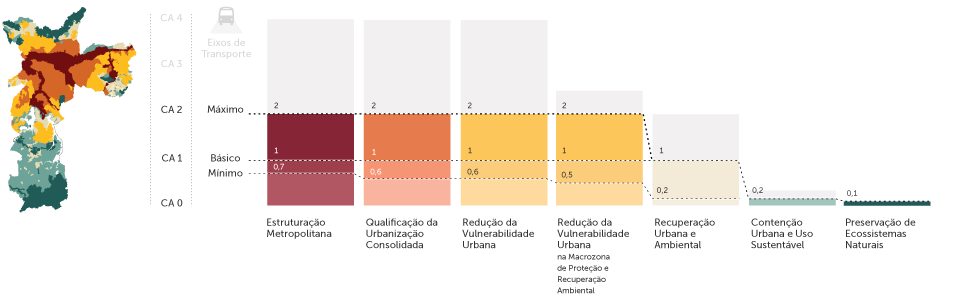
\includegraphics[width = \textwidth]{imagens/CA_macroareas.png}
    \end{subfigure}

    \caption*{\raggedright \textbf{Eixos de Estruturação da Transformação Urbana (EETU)}}
    \begin{subfigure}{.9\textwidth}
        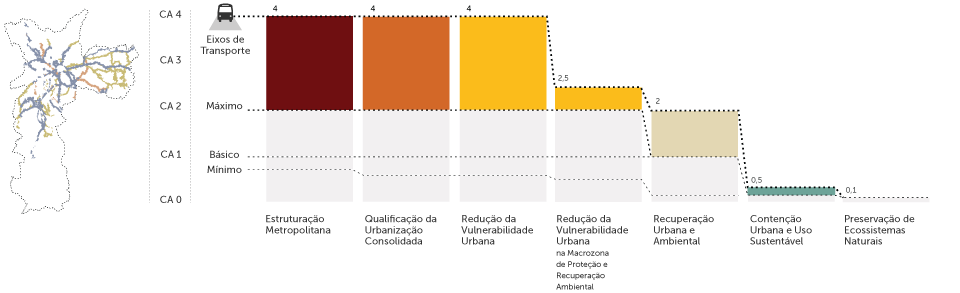
\includegraphics[width = \textwidth]{imagens/CA_eixos.png}
    \end{subfigure}
    \caption*{Fonte: \url{https://gestaourbana.prefeitura.sp.gov.br/marco-regulatorio/plano-diretor/entenda-o-projeto-de-lei-68813/}}
\end{figure}

No PDE, foram estabelecidos diferentes níveis de CA na cidade, a depender dos objetivos que se tem em relação à região, como é possível observar na Figura \ref{fig:CA}. Nas regiões de preservação ambiental, por exemplo, o CA máximo é de 0.1, o menor da cidade, enquanto nas áreas do entorno de equipamentos de transporte pública de alta capacidade, (EETUs), o CA deve estar entre 2 e 4. Com isso, o adensamento é direcinado às áreas próximas à infraestrutura de transporte público, com o objetivo de estimular seu uso. Nos EETUs, inclusive, não há limite de gabarito, diferentemente do resto da cidade, para também incentivar um padrão construtivo mais vertical.

Da mesma forma, existem parâmetros para a cota parte na cidade, a depender da localização. Nas Macrozonas de Estruturação e Qualificação Urbana, por exemplo, a cota parte apontada na Equação \ref{eq:cotaparte} como $Q$ equivale a 20. Em termos práticos, isso significa que um lote de 1.000m$^2$ hipotético deve apresentar no mínimo 50 unidades habitacionais. Este valor não é incrementado por um aumento do CA, mas pode decrescer se o CA escolhido pelo projeto seja menor do que o CA máximo da região.

\section{O problema}

Levando em consideração que um dos principais objetivos do PDE é estimular o adensamento de determinadas áreas, é importante avaliar se os intrumentos de regulação são capazes de definir a densidade populacional. Essa avaliação pode ser dividida em duas etapas, como demonstrado na Figura \ref{fig:proposta}. Na primeira, é necessário compreender se a regulação encontra repercussão nos padrões construtivos da cidade, o que está relacionado com o \textit{enforcement} da política e a resposta dos agentes aos incentivos. Por exemplo, na maioria dos EETUs, o CA a partir de 2014 deve estar entre 2 e 4, então na prática para uma mesma determinada configuração dada pela regulação, é possível se observar uma região com o dobro da densidade construtiva da outra. Ademais, quando se considera o mercado habitacional informal, é possível observar em uma área de preservação ambiental com CA máximo igual a 0,1, uma região urbanizada com o CA muito maior do que o permitido.

\begin{figure}[h]
    \centering
    \caption{Impacto dos instrumentos de regulação na densidade populacional}
    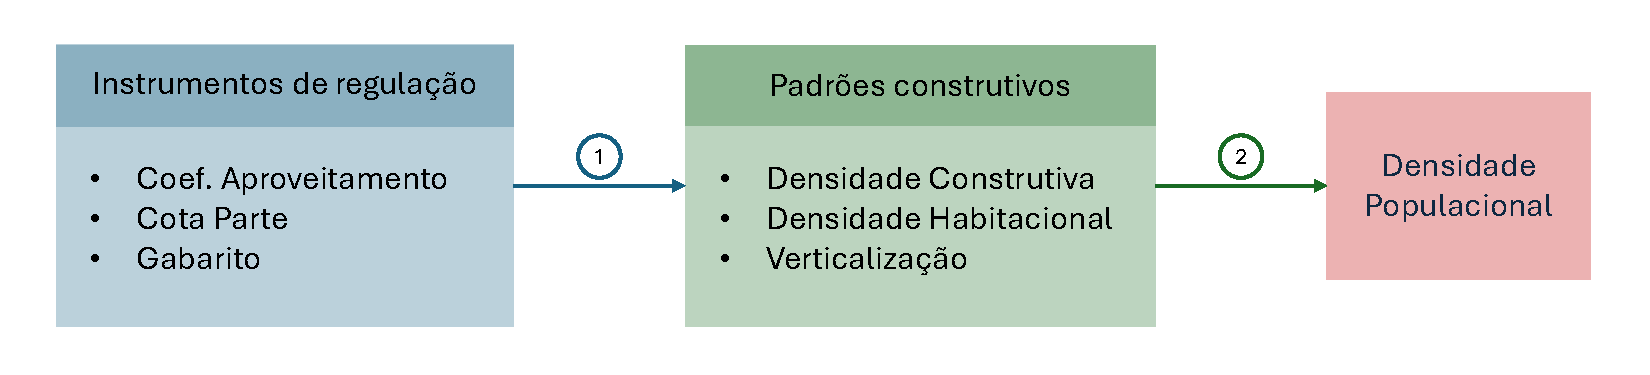
\includegraphics[width = \linewidth]{imagens/desenho_proposta.pdf}
    \label{fig:proposta}
\end{figure}

A segunda etapa foca em compreender se estes padrões construtivos de fato geram a densidade populacional que se espera. É esperado, por exemplo, que mais área construída gera maior densidade populacional. Entretanto, se ela estiver sendo alocada para poucas unidades habitacionais, talvez não seja observado um aumento na densidade. Nesse sentido, mesmo caso a regulação consiga definir perfeitamente o padrão construtivo, não necessariamente ela será capaz de definir a densidade populacional.

O escopo desta pesquisa é compreender se os padrões construtivos que estão sendo exigidos e incentivados pela regulação são capazes de gerar a densidade desejada. Para tanto, serão usados os dados do IPTU para identificar o padrão construtivo que se observa na cidade hoje e os dados do Censo de 2022 para identificar a densidade demográfica da cada região. A metodologia da manipulação de dados e estatísticas descritivas se encontram na Seção \ref{sec:dados}. Na Seção \ref{sec:analise} será medido os padrões construtivos são capazes de definir a densidade populacional. Por fim, na Seção \ref{sec:conclusao} serão trazidas as reflexões finais.


\chapter{Dados}
\label{sec:dados}

\section{Dados do Censo}

Para compreender o perfil geográfico da distribuição populacional de São Paulo foram utilizados os dados preliminares do Censo de 2022, feito pelo IBGE. Segundo o levantamento, a atual população do município de SP se encontra em 11.451.999 de habitantes, dividios em 4.996.529 de domicílios, dos quais apenas 4.316.336 estão ocupados. Na Figura \ref{fig:populacao} é possível observar quais são as áreas mais densas da cidade. A densidade foi calculada através da população no setor censitário dividida pela sua área. Os dados do censo foram utilizados em sua escala mais granular possível: nível setor censitário. 

\begin{figure}[!h]
    \centering
    \caption{Densidade populacional em São Paulo por setor censitário (Censo 2022)}
    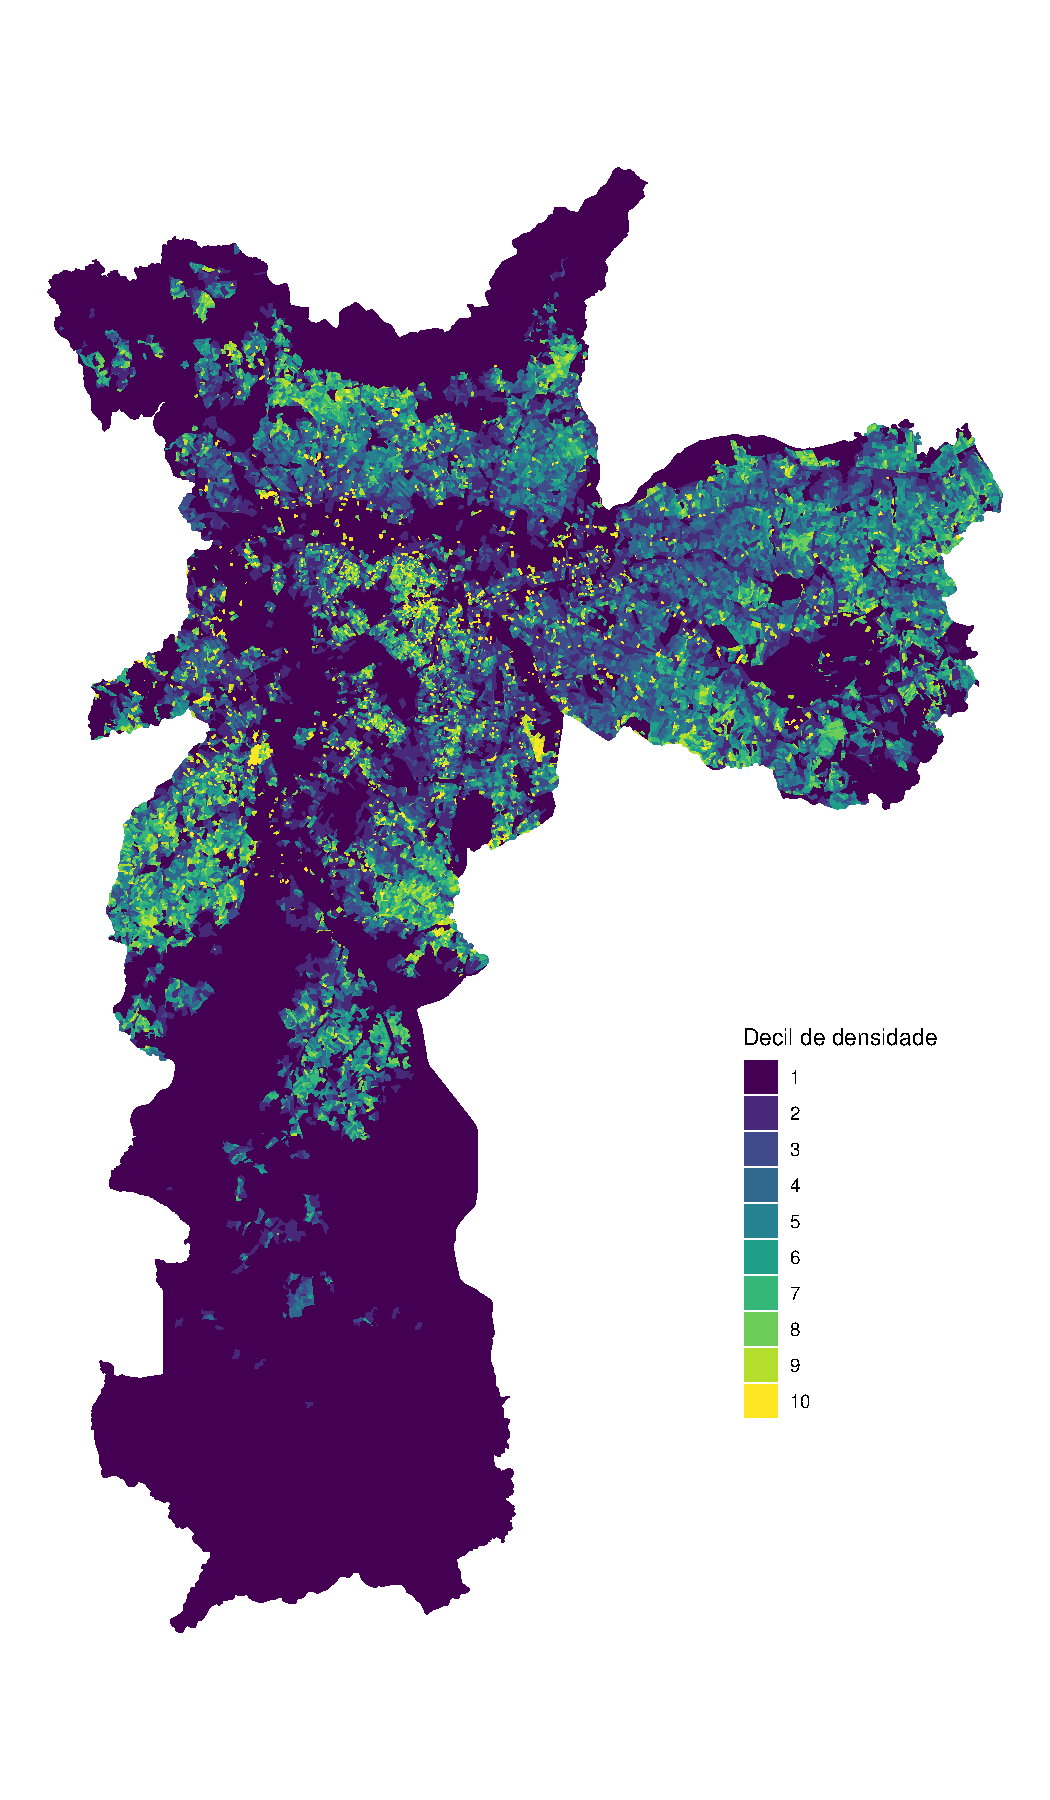
\includegraphics[width = .85\linewidth]{imagens/mapa.pdf}
    \label{fig:populacao}
\end{figure}

A metodologia para a delimitação dos setores censitários leva em consideração diversos fatores, como elementos na paisagem que se constituam em barreiras naturais ou artificiais e dificultam o trabalho do agente, pontos de referência estáveis e de fácil identificação no terreno, limites das estruturas territoriais, entre outros \cite{IBGE2024}. De maneira geral, estes limites são construídos de forma que o agente de coleta consiga cobrir o setor inteiro, minimizando os erros de medição. Estes setores censitários também são georreferenciados através da malha preliminar divulgada pelo IBGE e apresentam um número de identificação que contém o município, distrito, subdistrito e setor da região.

É interessante notar na Figura \ref{fig:populacao}, que o clássico modelo, no qual população se concentra principalmente no centro apresenta mérito, dado que perto da região da Sé, centro histórico de São Paulo, há uma enorme concentração populacional. Entretanto, é surpreendente a densidade populacional nas favelas de Paraisópolis e Heliópolis, que acabam por ser as áreas mais densas da cidade. Na Figura \ref{fig:dens-distcentro} é possível ver como ainda que haja uma relação entre a densidade populacional e a distância, ela não é tão perfeita quanto no modelo microeconômico. Paraisópolis, por exemplo, está a 15km do centro e ainda é a região mais densa de São Paulo -- mais detalhes serão discutidos adiante.

\begin{figure}[h]
    \centering
    \caption{Densidade populacional na medida em que se distancia da Sé}
    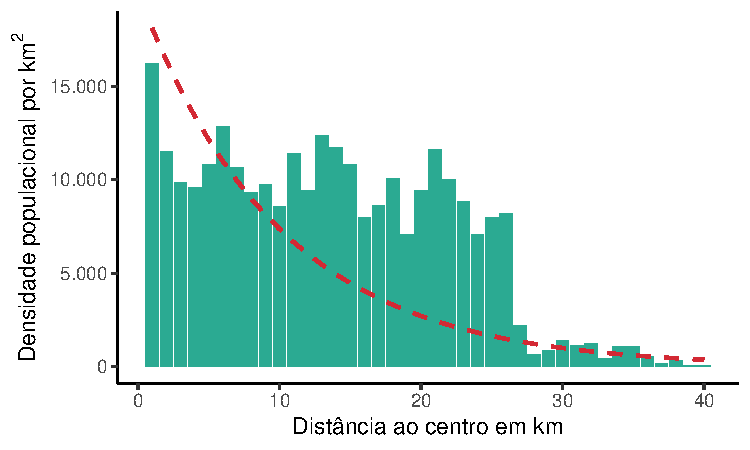
\includegraphics[width = .75\linewidth]{imagens/densidade_distcentro.pdf}
    \label{fig:dens-distcentro}
\end{figure}

\section{Dados do IPTU}

Em relação aos dados sobre os empreendimentos imobiliários, a base de dados escolhida foi do IPTU. Para os fins deste artigo, ela é a mais completa, visto que não representa um fluxo de novos imóveis construídos todos os anos como a base da Embraesp, mas apresenta um estoque imobiliário de tudo que já foi construído legalmente na cidade. Dito isso, estão cadastrados os 3.096.719 números únicos de contribuintes, que, segundo a definição da documentação dos dados no GeoSampa, ``A cada imóvel urbano corresponderá um número de inscrição no Cadastro Imobiliário Fiscal, entendendo-se como imóvel: I - a área de terreno, construído ou não, definida em matrícula do competente Serviço de Registro de Imóveis ou em transcrições ainda vigente''. Os únicos dados que não constam nessa base são relativos a lotes irregulares ou não registrados, como em áreas de favelas. 

Entre os dados disponíveis do IPTU, se destacam a área do terreno, a área construída, a área ocupada e o número de pavimentos do empreendimento. O tipo de uso do imóvel também está disponível, mas como esta pesquisa foca em densidade populacional, foram descartados os usos não residenciais.  Logo, com estes dados é possível identificar os padrões construtivos na cidade, mantendo os cálculos os mais fiés possível à forma como são calculados pela regulação. A densidade construída, por exemplo, é definida pelo CA observado na construção -- não é considerando nesta análise o CA regulado da região. A distribuição destes indicadores pode ser vista na Figura \ref{fig:histogramas}.

\begin{figure}[h]
    \centering
    \caption{Distribuição do padrão construtivo em cada lote residencial de São Paulo}
    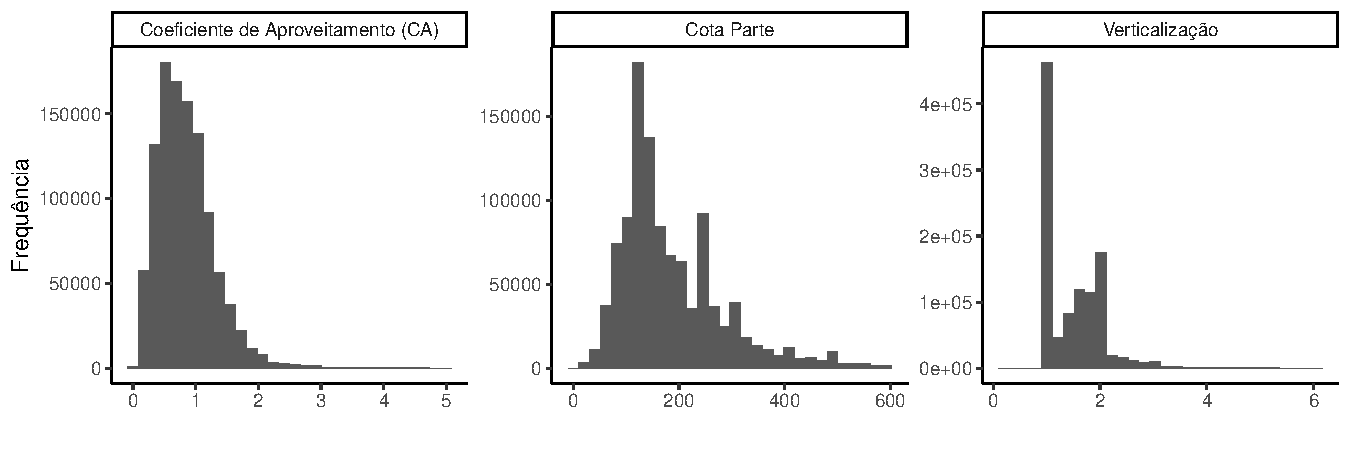
\includegraphics[width = \linewidth]{imagens/indicadores.pdf}
    \label{fig:histogramas}
\end{figure}

Na Figura \ref{fig:area_construida}, é possível observar a distribuição da área construída por tipo e padrão de uso. Em São Paulo, 70\% da área construída é residencial, sendo que o padrão residencial mais comum é o "C". O padrão é uma divisão feita no cálculo do IPTU \cite{lei10235_1986}, para criar descontos do imposto para imóveis com características desejáveis do ponto de vista do planejamento urbano, como maior adensamento, ou para menor poder aquisitivo. Medidas como metragem, pé direito, vaga de garagem, número de pavimentos, elementos arquitetônicos, materiais de construção, etc., são fatores levados em consideração para determinar o padrão. No caso do "C", ele está no meio da escala de densidade, sendo "A" o mais denso, e "E" o menos. O segundo uso mais comum é o comercial, seguido do industrial e entretenimento. Na categoria de entretenimento, se encontram templos religiosos, clubes, estádios esportivos, cinemas, aeroporto, museu, zoológico, entre outros.

\begin{figure}[h]
    \centering
    \caption{Área construída no município de São Paulo por tipo e padrão de uso}
    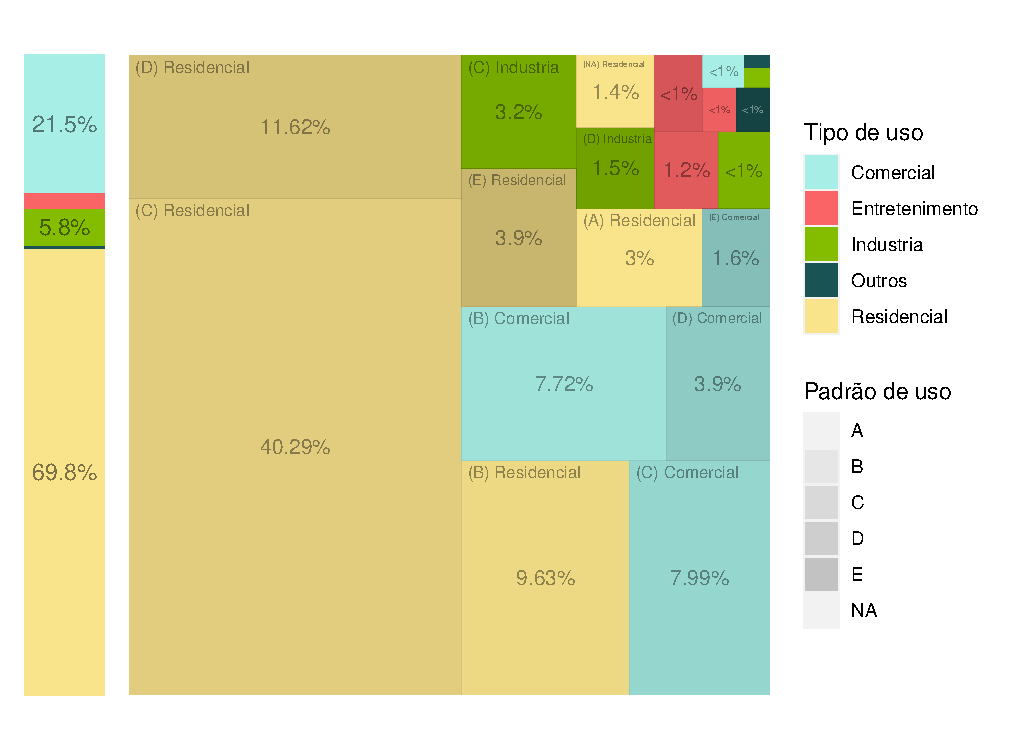
\includegraphics[width = .8\linewidth]{imagens/tree_area_construida.pdf}
    \label{fig:area_construida}
\end{figure}

De fato, ao observar os indicadores na Figura \ref{fig:histogramas}, é possível notar que o perfil habitacional de São Paulo é bastante horizontal. É surpreendente que 95\% dos lotes residenciais em São Paulo apresentam 2 ou menos pavimentos. Ainda, a mediana do CA observado é 0,8, o que indica que em mais da metade dos lotes da cidade foi construído menos do que a área do terreno. Ainda, a cota parte observada mediana dos lotes da cidade é de 155$m^2$, o que representa um uso do terreno para poucas unidades habitacionais em média. 

\begin{figure}[h]
    \centering
    \caption{Variação no tempo dos padrões construtivos residenciais observados em São Paulo}
    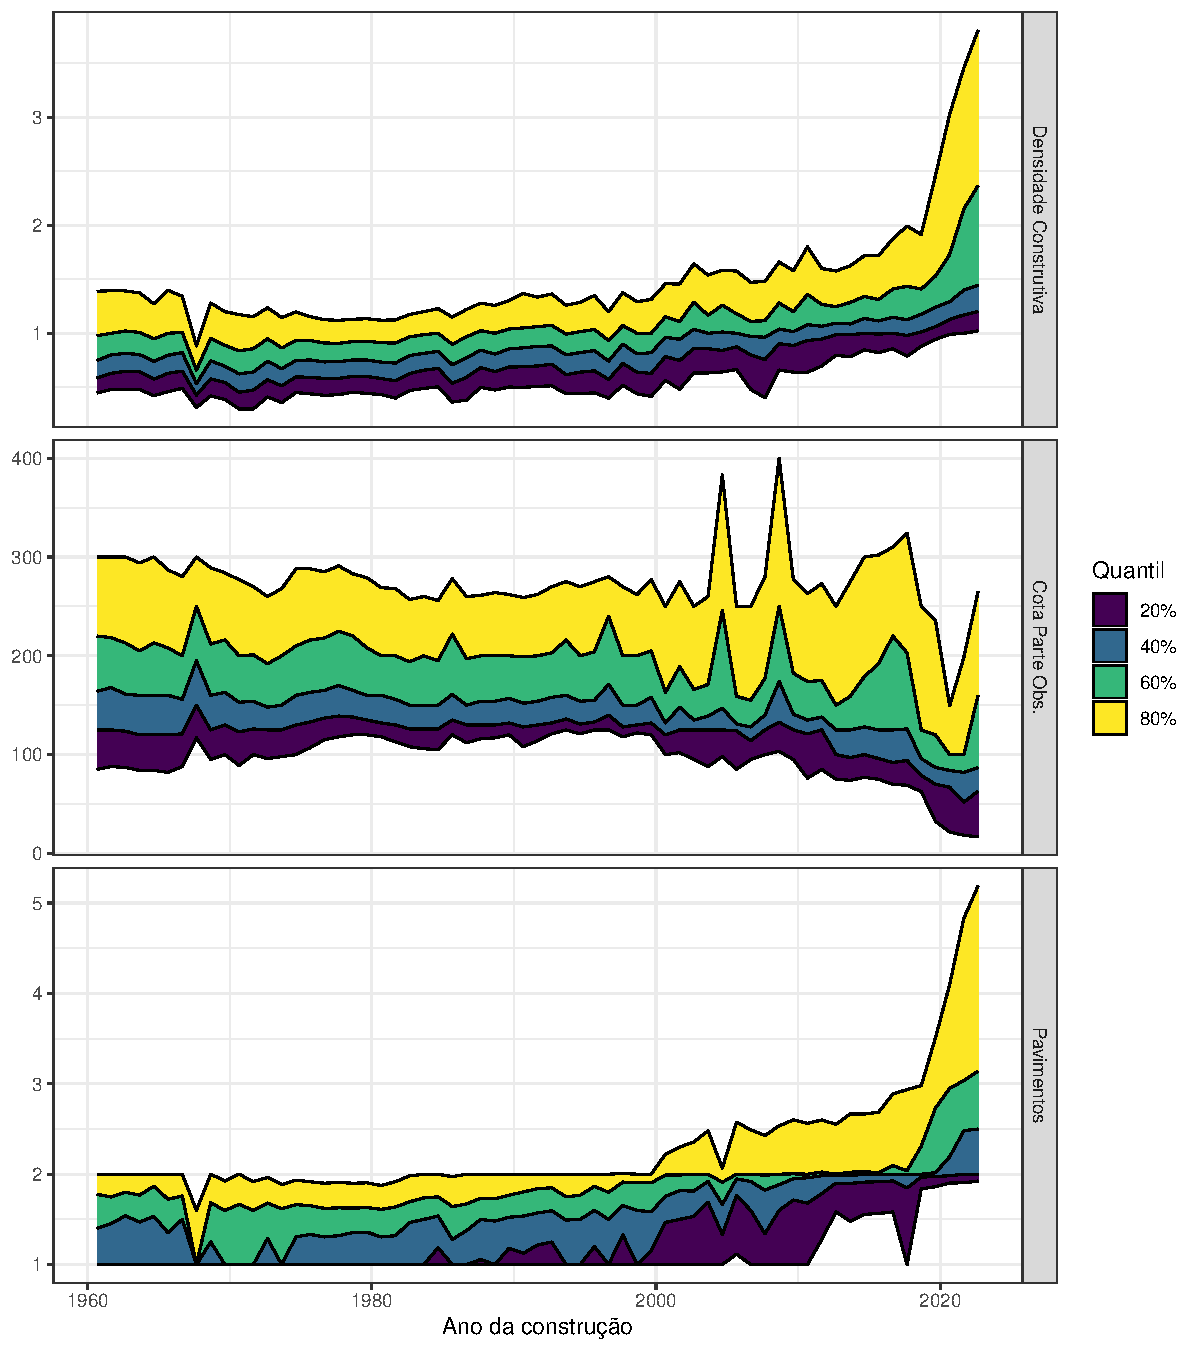
\includegraphics[width = \linewidth]{imagens/indicadores_tempo.pdf}
    \label{fig:indicadores-tempo}
\end{figure}

Todavia, ao analisar estes indicadores ao longo do tempo na Figura \ref{fig:indicadores-tempo}, fica evidente a trajetória de adensamento. Na figura, cada linha representa um quantil dos lotes do IPTU. Ao ordenar as construções no ano 2020 de maneira crescente de CA observado, o empreendimento na posição 80\% dessa fila apresenta um CA observado de 3,8. Este mesmo procedimento nos anos 2000 retornaria um empreendimento com CA observado igual a 1,46. Analogamente, a cota parte observada que em 2020 apresenta o quantil 20\% de meros 21,7 metros quadrados, no ano 2000 apresentaria 100 metros quadrados. Isso evidencia que nos últimos anos São Paulo passou por um forte processo de adensamento.

\section{Cruzamento dos dados}

Os dados do IPTU não são georreferenciados, então desacompanhados de outros dados não é possível cruzá-los com os do Censo. O que possibilita fazer essa junção é que o número único de contribuinte do IPTU, também é o código do Setor, Quadra e Lote (SQL) que o empreendimento se encontra. Nesse sentido, é possível decompor o SQL e cruzar com as bases de lotes, quadras e setores do GeoSampa, que contêm a geometria de cada  um dos 1.677.980 lotes, 45.987 quadras e 309 setores da cidade. O que explica a diferença entre o número de lotes e número de números dos contribuintes são os lotes que contém um condomínio, que pode haver diversos números únicos de contribuintes em apenas um lote. Nos dados de IPTU, há 1.314.353 contribuintes em lotes com apenas uma unidade habitacional e 33.129 condomínios, que contêm 1.782.366 unidades. Ao cruzar o SQL do IPTU com a base de lotes, 44.319 contribuintes não encontram um par na outra base, o que representa uma perda de 1,67\% das unidades. Caso o join seja feito com a base de quadras, a perda passa a ser de 820 contribuintes, um erro de 0,03\%. Já quando são cruzados com base no setor, o erro chega a 0.

Agora, com os dados do censo georreferenciados e os dados do IPTU também georreferenciados, é necessário juntar estas bases. Entretanto, como o recorte dos setores censitários não respeita os recortes dos lotes, algum tipo de critério deve ser adotado para conectar essas geometrias. Duas abordagens foram feitas, a primeira com um join geográfico e a segunda, a partir da rasterização de ambos os dados. Na primeira, para cada um dos 27.592 setores censitários foram identificados todos os lotes que se interseccionam com os setores. A partir disso, foram cortados os lotes que não estão contidos apenas em um setor, de forma a atribuir seus dados a todos os setores que pertence, ponderado pelo percentual de sua área que intersecciona com cada setor. A segunda abordagem envolve dividir a cidade em um quadriculado (\textit{raster}) e converter tanto os dados do IPTU quanto do censo para esta escala. A metodologia é parecida, visto que formado o quadriculado, os lotes são dividos entre cada quadrado, ponderando-se pelo percentual de sua área que intersecciona com cada um.

Dessa forma, para cada setor censitário ou para cada célula do \textit{raster}, há varios lotes, que devem ser agregados segundo algum critério. Para a área construída, área ocupada, área do terreno e unidades, os valores de cada lotes podem ser simplesmente somados. Entretanto, no caso da verticalização fica mais complicado e é necessário estabelecer de maneira muito clara a metodologia de cálculo, que é pouco documentada e unificada na literatura \cite{ccalicskan2022morphological}. Diversas métricas são possíveis para agregar o número de pavimentos de uma região, mas muitas delas podem gerar erros de medição ou acabar representando uma medida muito semelhante ao CA. Mais detalhes são discutidos no Apêndice \ref{appendix:verticalizacao}.

Com as bases relacionadas, é importante fazer um balanço para analisar se as informações batem. A única informação em comum entre as bases é o número de unidades habitacionais, que nos dados do IPTU são classificadas como unidades, e na do Censo como domicílios. A definição deles não é exatamente a mesma, porém é a única informação possível de ser validada. Caso o número de domicílios no Censo seja maior do que o de unidades no IPTU, é um forte indicativo de que há moradias irregulares. Para medir essa diferença, foi criado um espectro de irregularidade, que é construído a partir do número de unidades dividido pelo número de unidades mais domicílios. Caso o valor calculado seja próximo de 50\%, as informações são consistentes, ou seja, o número de unidades do IPTU é igual ao número de domicílios no censo. Na medida em que o balanço se aproxima de 0\%, significa que há mais unidades no censo do que no IPTU, enquanto mais próximo de 100\% indica o contrário.

\begin{quote}
    ``Domicílio é o local estruturalmente separado e independente que se destina a servir de habitação a uma ou mais pessoas, ou que esteja sendo utilizado como tal. A separação fica caracterizada quando o local de habitação for limitado por paredes, muros ou cercas e coberto por um teto, permitindo a uma ou mais pessoas, que nele habitam, isolar-se das demais, com a finalidade de dormir, preparar e/ ou consumir seus alimentos e proteger-se do meio ambiente, arcando, total ou parcialmente, com suas despesas de alimentação ou moradia. A independência fica caracterizada quando o local de habitação tem acesso direto, permitindo a seus moradores entrar e sair sem necessidade de passar por locais de moradia de outras pessoas'' \cite{IBGE2013}.
\end{quote}

\begin{figure}[h]
    \caption{Inconsistências entre dados do IPTU e do censo}
    \centering
    \begin{subfigure}{.8\linewidth}
        \centering
        \caption{Diferença entre unidades e domicílios por setor censitário}
        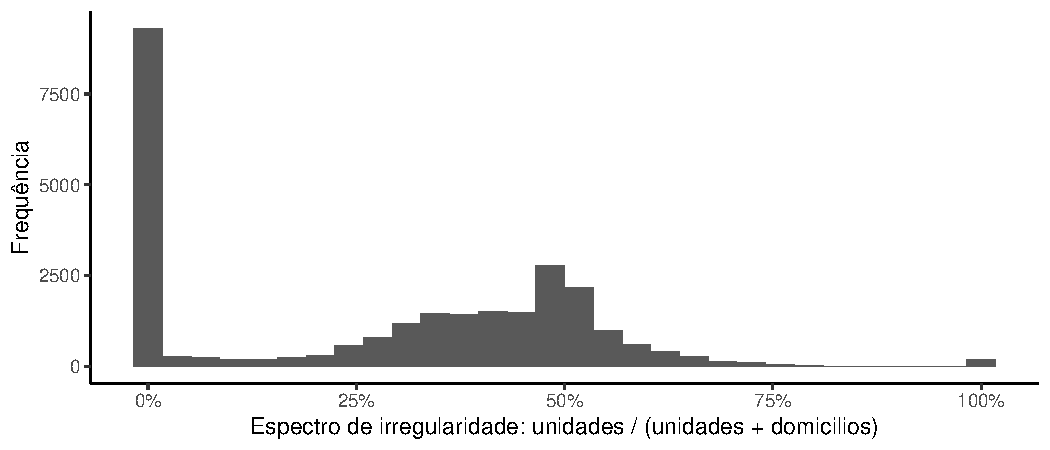
\includegraphics[width = \linewidth]{imagens/disparidade_censoIPTU.pdf}
        \label{fig:balanco}
    \end{subfigure}
    \begin{subfigure}[t]{0.45\linewidth}
        \caption{Abordagem join}
        \centering
        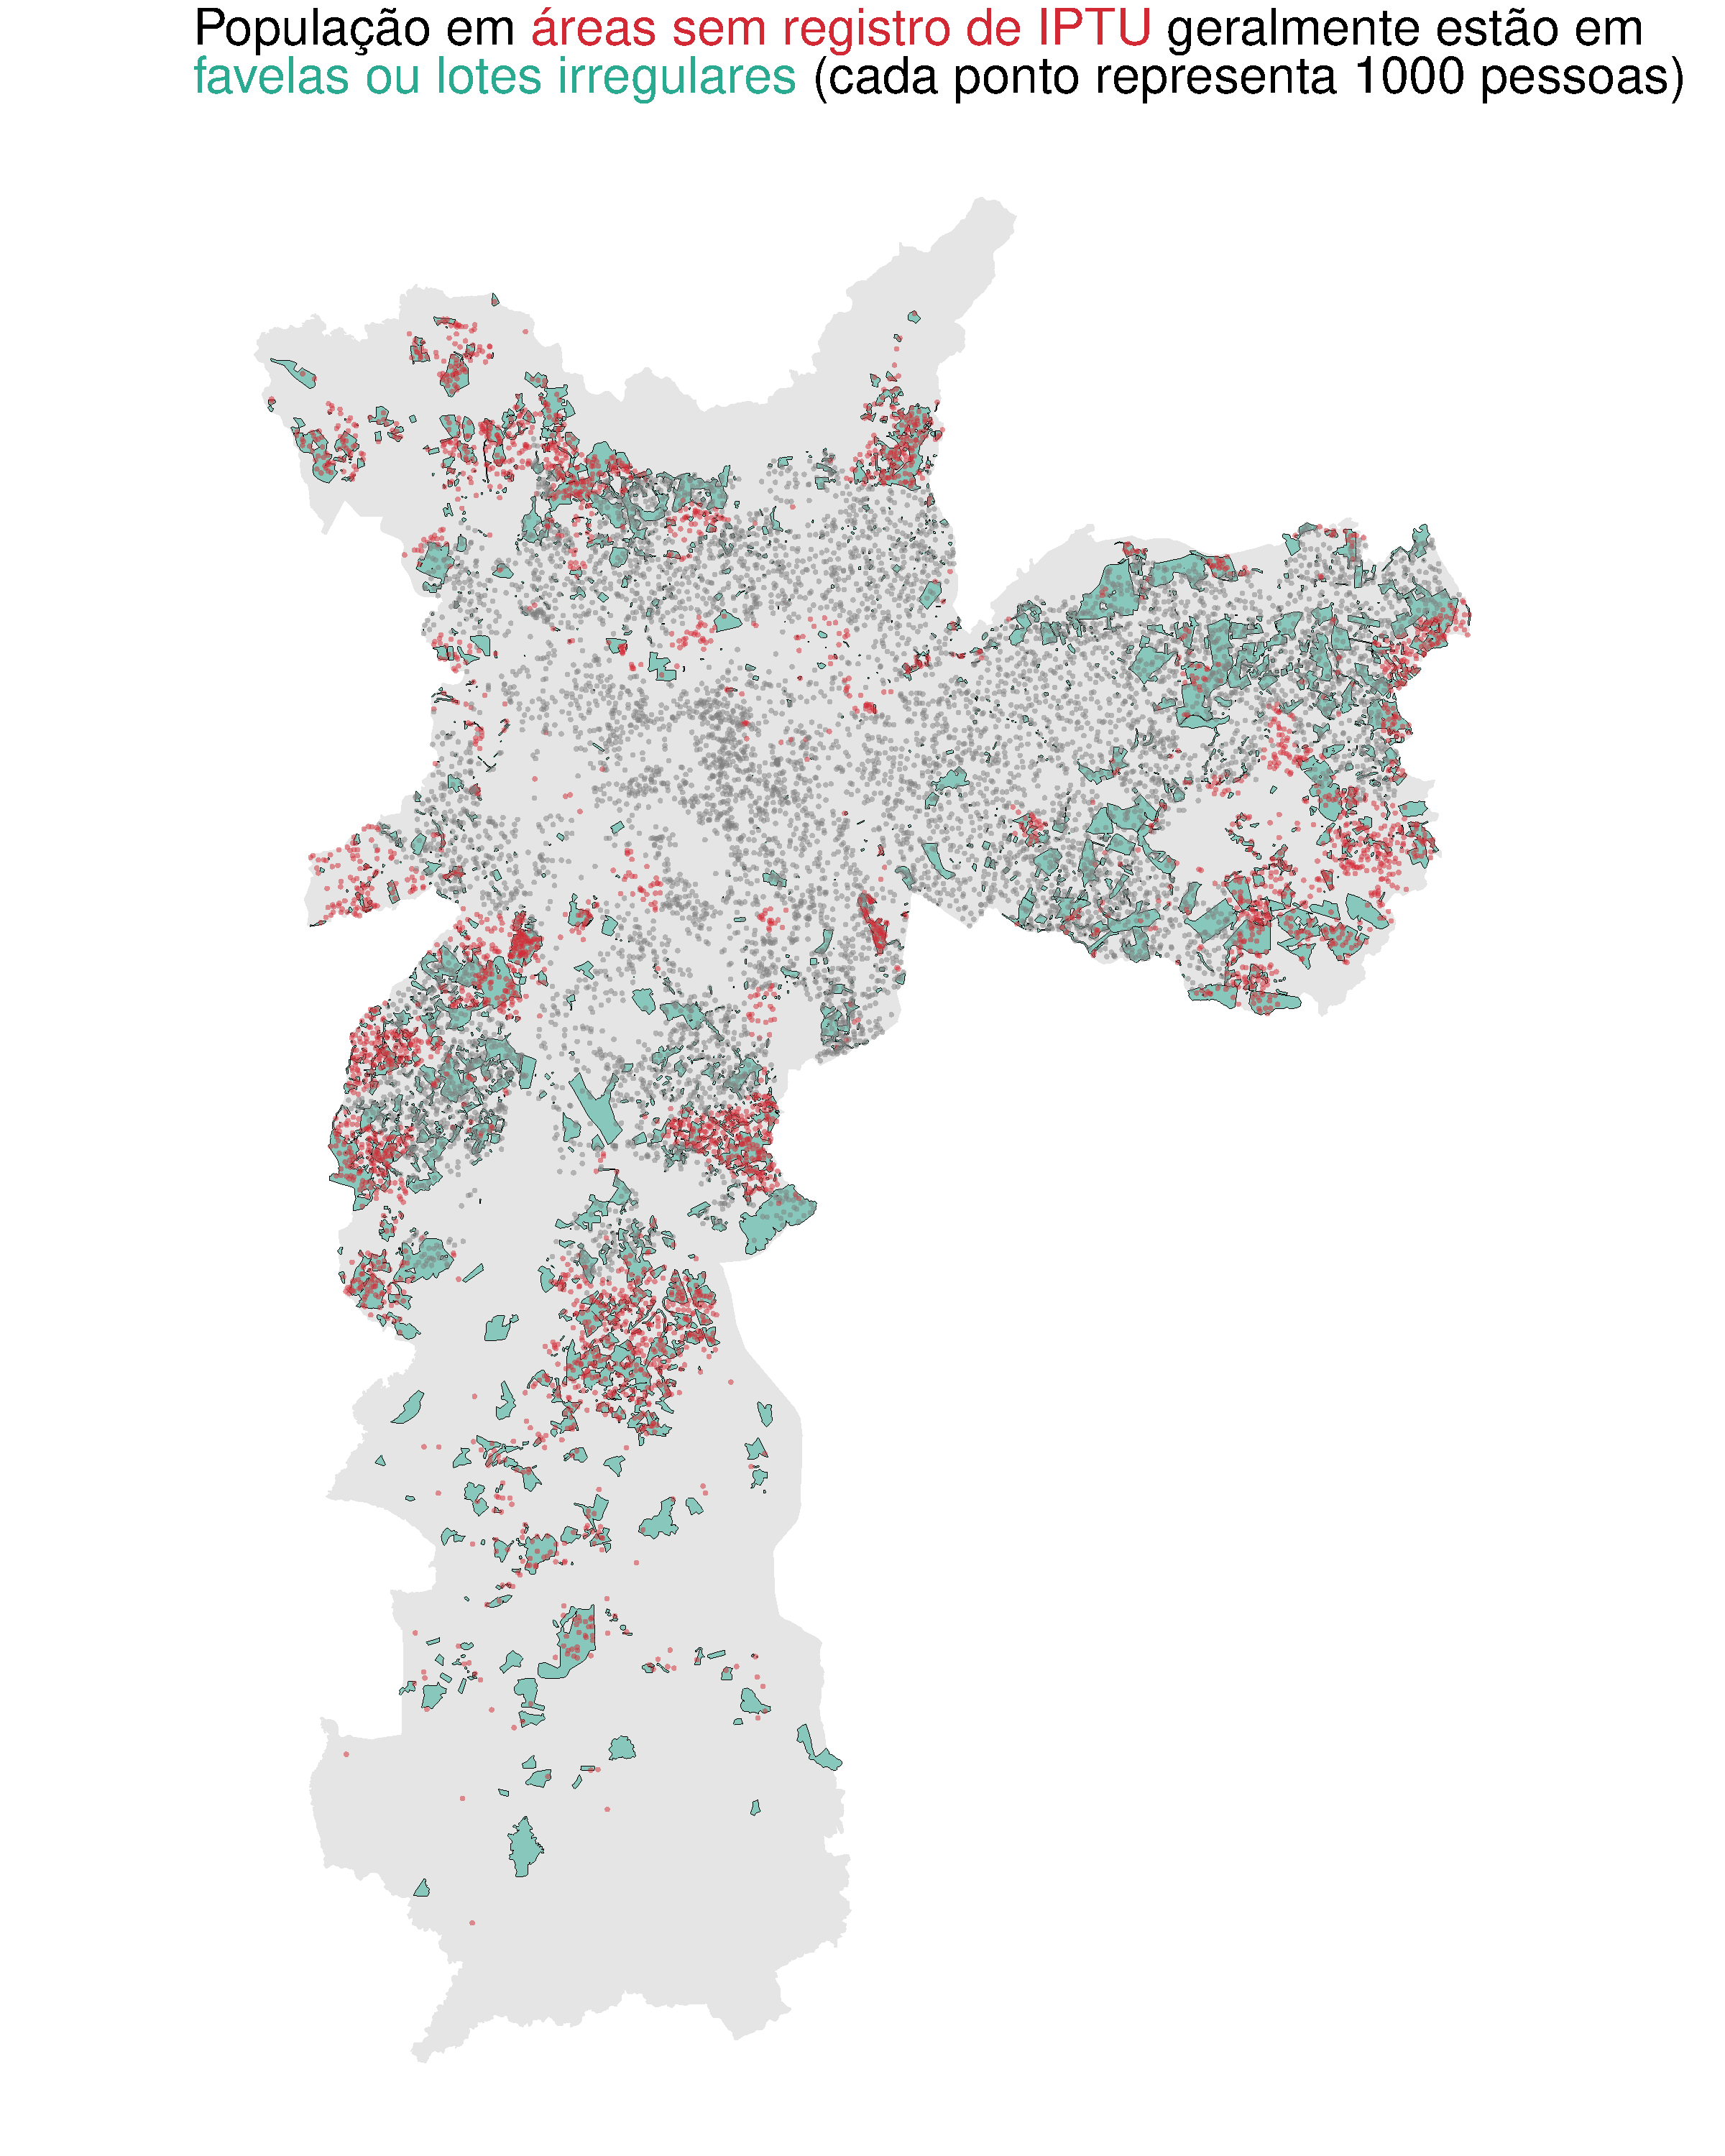
\includegraphics[width = \linewidth]{imagens/mapa_pontos.pdf}
        \label{fig:pontos_erro}
    \end{subfigure}
    \hfill
    \begin{subfigure}[t]{0.45\linewidth}
        \caption{Abordagem \textit{Raster}}
        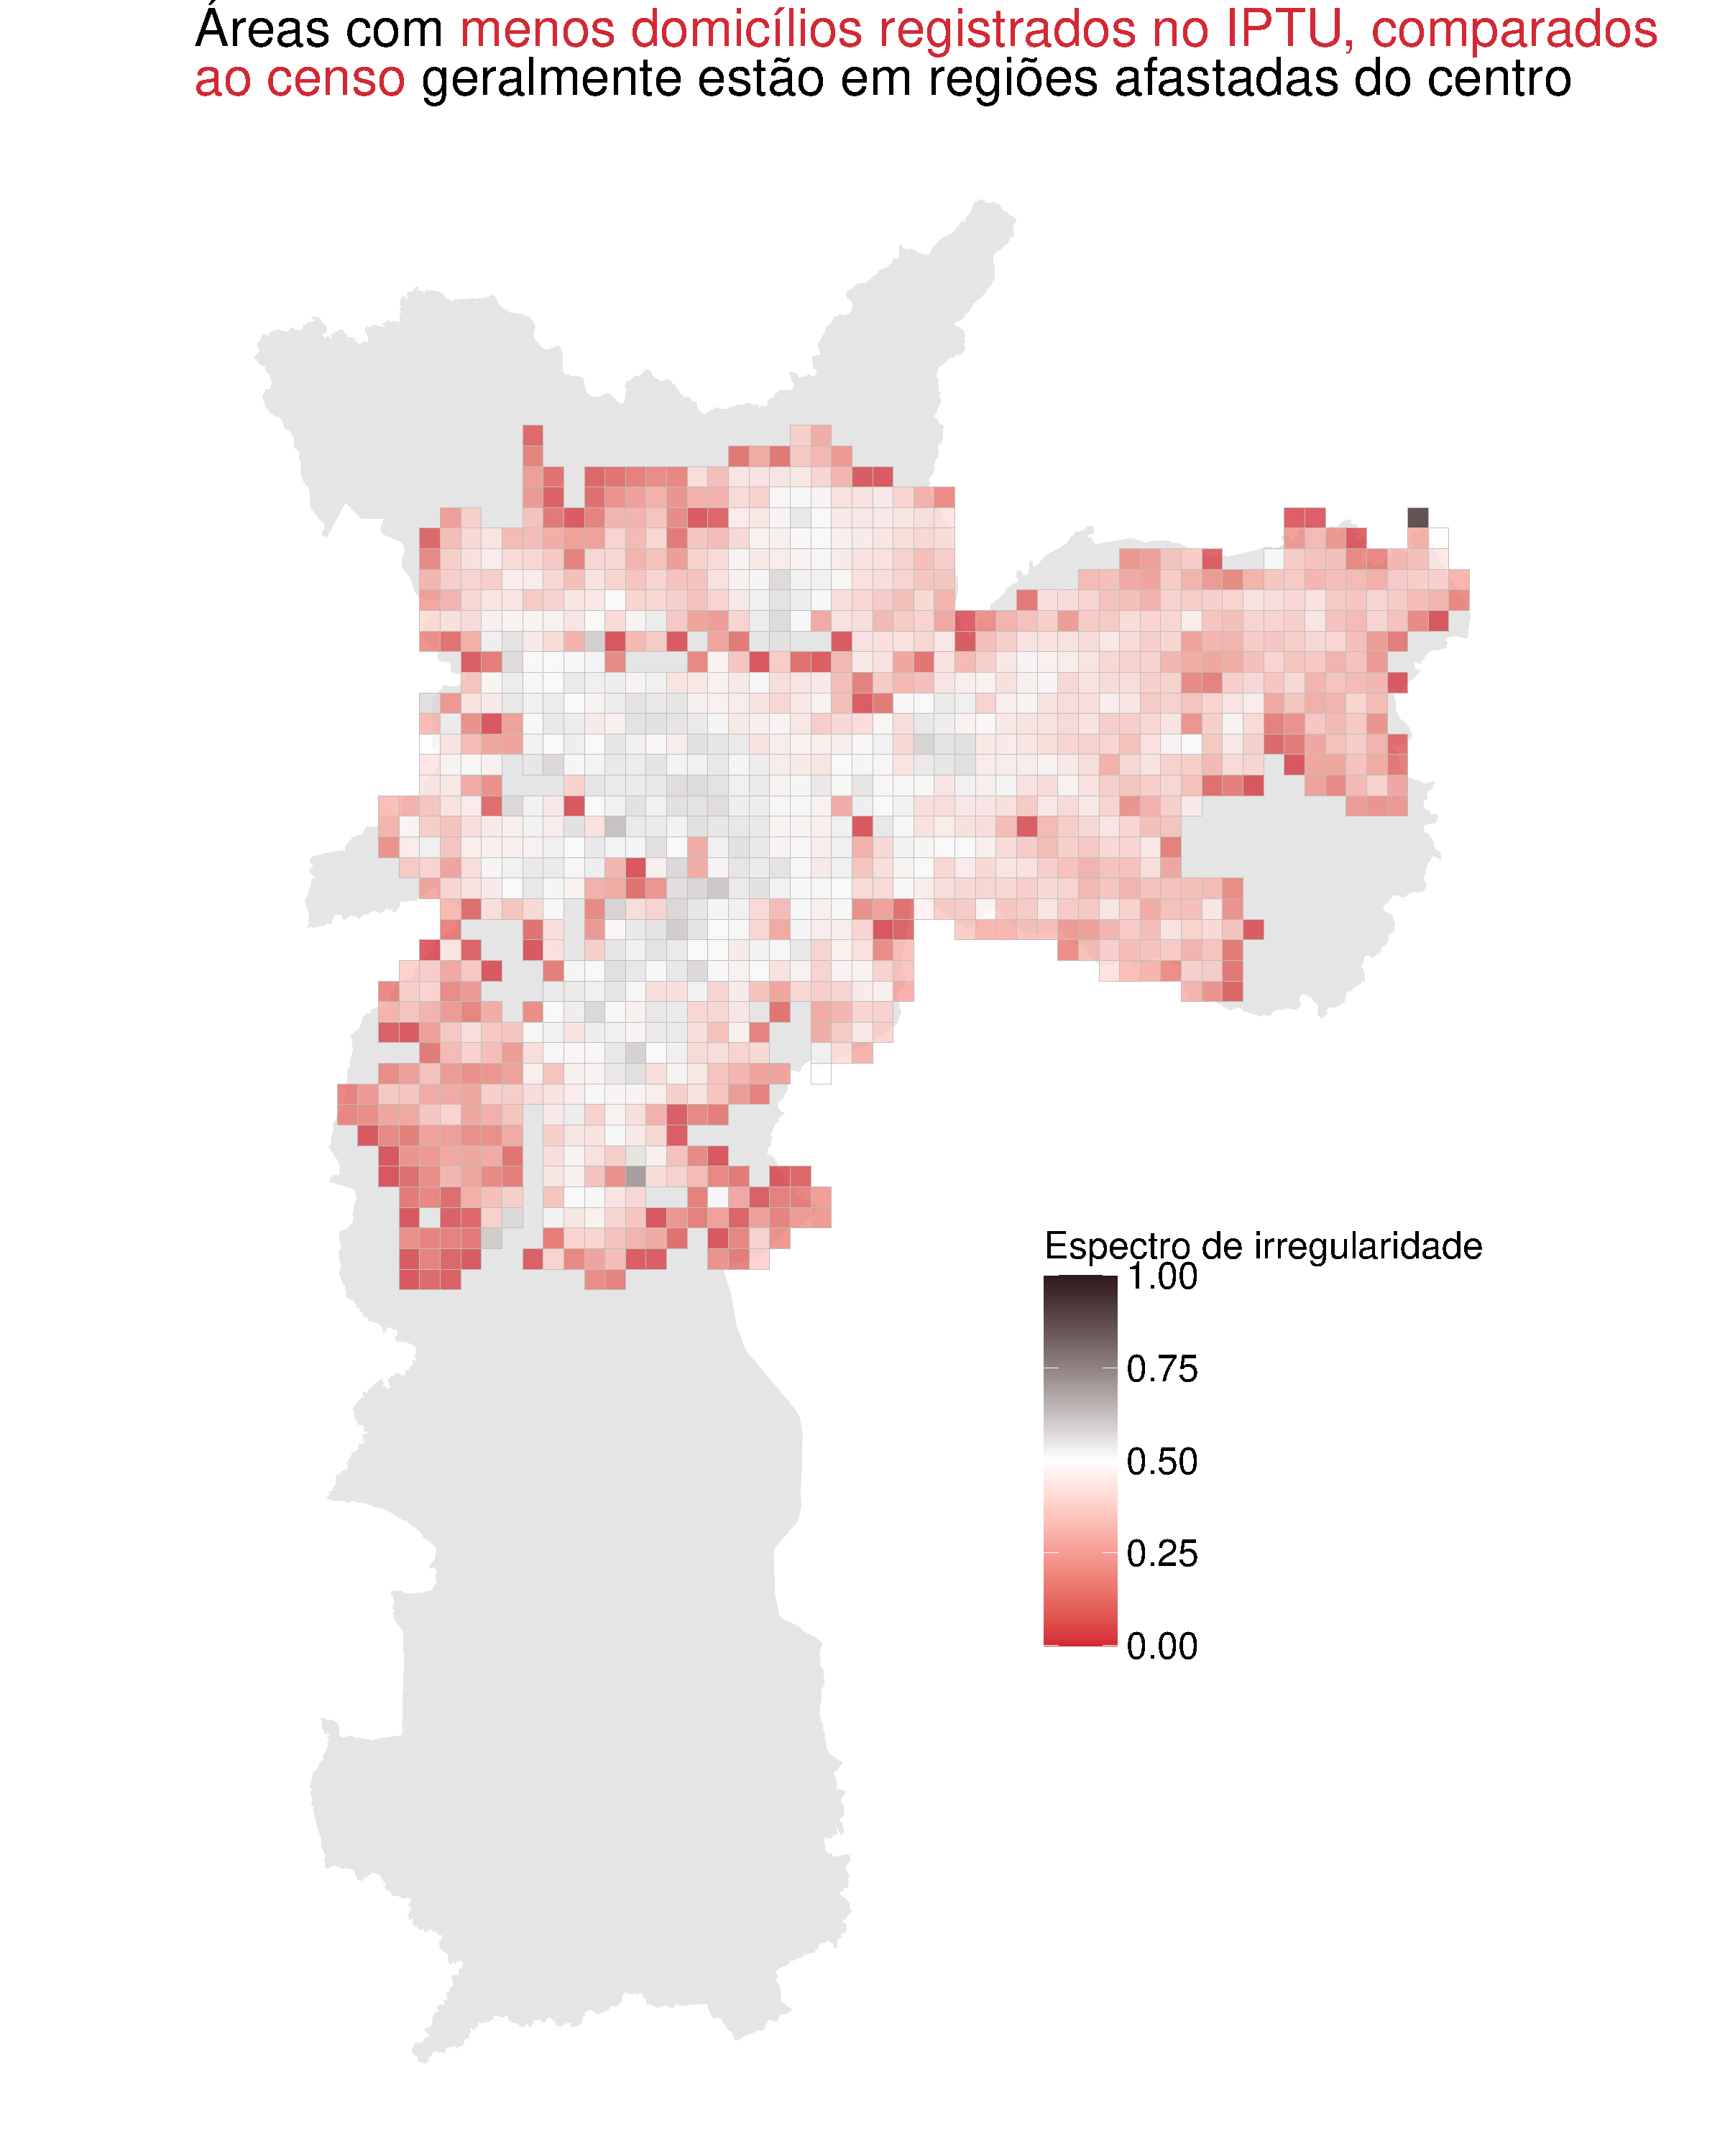
\includegraphics[width = \linewidth]{imagens/balanco_raster.pdf}
        \label{fig:balanco-raster}
    \end{subfigure}
    \label{fig:erros-join}
\end{figure}

Para analisar em termos práticos, no histograma da Figura \ref{fig:balanco} é possível identificar que há diversos setores censitários com domicílios registrados, mas nenhuma unidade habitacional no IPTU. Ademais, são incomuns os casos em que são semelhantes os números de domicílios e unidades. No mapa da Figura \ref{fig:pontos_erro}, para cada setor censitário foram simulados pontos aleatórios dentro da geometria do setor para representar sua população. Nos setores censitários em que não há nenhum lote presente, ou seja, há uma subnotificação de imóveis na base do IPTU, os pontos foram pintados de vermelho. Em azul, estão as geometrias de lotes irregulares e favelas, disponibilizados no GeoSampa. É possível identificar que a maioria dos setores censitários que não possuem loteamento estão nessas áreas de lotes irregulares e favelas.  Na Figura \ref{fig:balanco-raster}, um procedimento semelhante foi feito. Para cada célula do \textit{raster} foi calculado este indicador de irregularidade para analisar as inconsistências entre as bases. É notável que as células que se encontram em regiões centrais apresentam uma quantidade pequena de erros. Os casos mais críticos são células nas periferias.

\begin{table}[h]
    \begingroup
\fontsize{9.8pt}{11.7pt}\selectfont
\begin{longtable}{lrrrrr} 
\caption{Células do \textit{raster} que apresentam a maior densidade populacional}
\label{tab:top5}\\
\toprule
 & \multicolumn{4}{c}{Favelas} &  \\ 
\cmidrule(lr){2-5}
Variável & 1. Paraisópolis & 2. Heliópolis  & 4. Paraisópolis & 5. Heliópolis & 3. Sé (Bela Vista) \\ 
\midrule\addlinespace[2.5pt]
População & 29.598 & 25.280 & 23.824 & 22.920 & 24.576 \\ 
Domicílios (Censo) & 11.655 & 10.178 & 9.361 & 9.001 & 17.875 \\ 
Domicílios Ocupados & 10.791 & 9.269 & 8.810 & 8.274 & 13.732 \\ 
Unidades (IPTU) & 0 & 1.857 & 7 & 3 & 21.057 \\ 
Espectro irregularidade & 0.00\% & 15.43\% & 0.08\% & 0.03\% & 54.09\% \\ 
Densidade populacional & 46.247 & 39.500 & 37.225 & 35.813 & 38.400 \\ 
Área & 640.000 & 640.000 & 640.000 & 640.000 & 640.000 \\ 
\bottomrule
\end{longtable}
\endgroup


\end{table}

Na Tabela \ref{tab:top5} estão descritas as 5 células do \textit{raster} que apresentam maior densidade populacional. É interessante observar que 4 das 5 regiões mais densas da cidade são de territórios de favelas e repletos quase completamente de domicílios que não estão registrados no IPTU. A densidade populacional do município de São Paulo no geral é de 7.529 habitantes por quilômetro quadrado, o que significa que esta célula do \textit{raster} posicionada na região de Paraisópolis apresenta uma densidade quase quatro vezes maior do que o resto da cidade. Outro fator interessante é o número maior de unidades no IPTU na região da Sé, se comparadas com domicílios do censo. Esta é uma das poucas regiões em que o espectro de irregularidade ultrapassa 50\%. Isso pode estar associada a alta taxa de abandono, que dificulta a medição por parte dos entrevistadores -- os dados do Censo indicam que 34,8\% dos domicílios estão desocupados.

Na Figura \ref{fig:rasters} é possível analisar o perfil geográfico dos padrões construtivos. Como é de se esperar, regiões com maior adensamento populacional também apresentam maior CA, verticalização e menor cota parte observados. É importante destacar que quanto mais lotes irregulares há em uma região, menos confiáveis são os padrões construtivos calculados, visto que estes são inteiramente calculados com base nos dados do IPTU, que são disponíveis apenas para lotes regulares.

\begin{figure}[h]
    \centering
    \caption{Distribuição geográfica dos padrões construtivos e densidade populacional}
    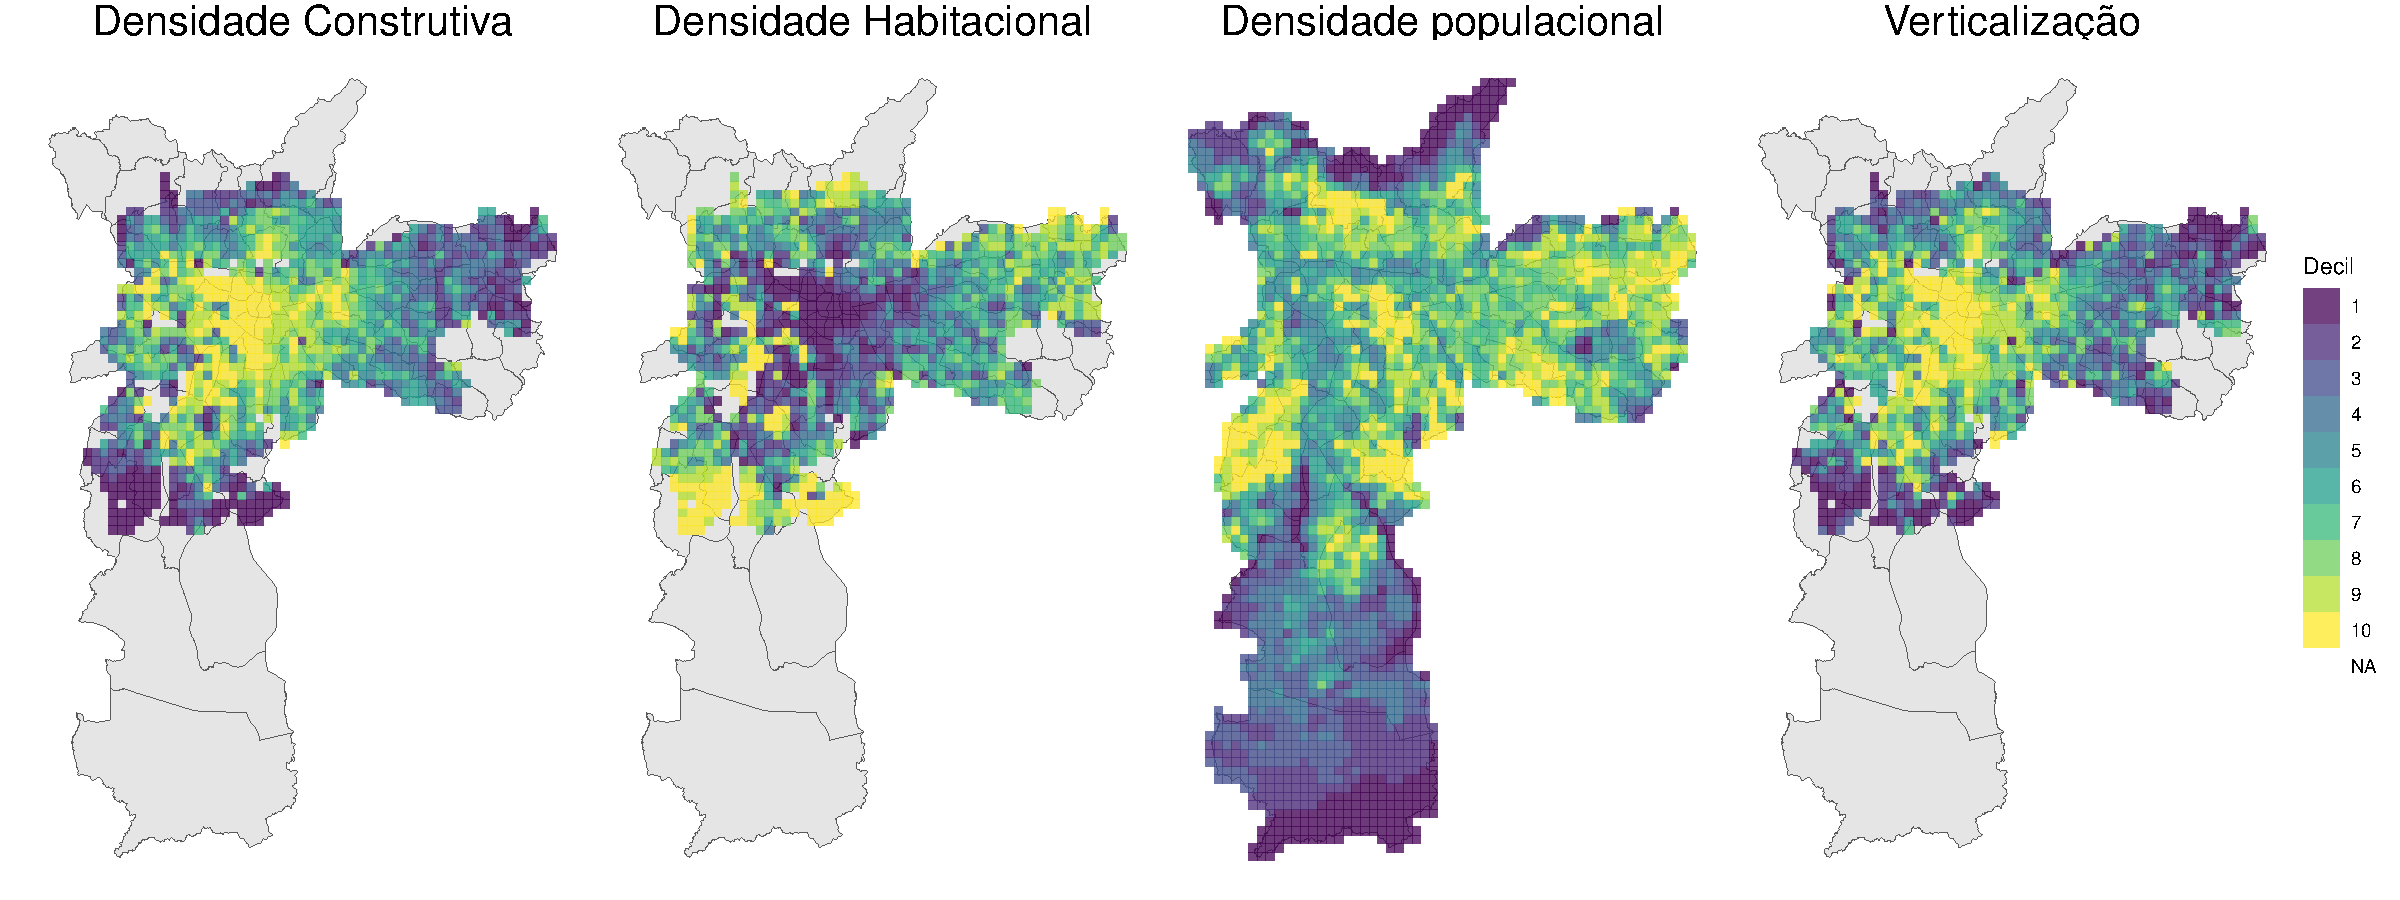
\includegraphics[width = \linewidth]{imagens/rasters_wide.pdf}
    \label{fig:rasters}
\end{figure}

Retomando a discussão sobre métricas de tipomorfologia, é importante definir com clareza o significado de densidade populacional \cite{ccalicskan2022morphological}. Em termos mais abrangentes, é a soma da população que se encontra em uma área. Todavia, a definição da área pode ser subjetiva. Por exemplo, se há um bairro que contém um lago, mas em toda a área de terra há um grande número de pessoas, a densidade será diluída se for considerada a área do lago. Nesse sentido, foram construídas duas métricas de densidade, uma densidade residencial que computa apenas a área de terreno de lotes residenciais, e a área total, que considera tudo, incluindo usos do solo não residenciais. Até este momento do artigo, a medida de densidade utilizada foi a total, mas na Seção \ref{sec:analise} essa diferenciação torna-se importante para avaliar os resultados. Os resultados para Figura \ref{fig:rasters} utilizando a densidade residencial podem ser observados no Apêndice \ref{appendix:rasters-corte}.

\begin{figure}[!h]
    \centering
    \caption{Matriz de correlação entre as variáveis de interesse -- espectro irregularidade entre 40 e 60\%}
    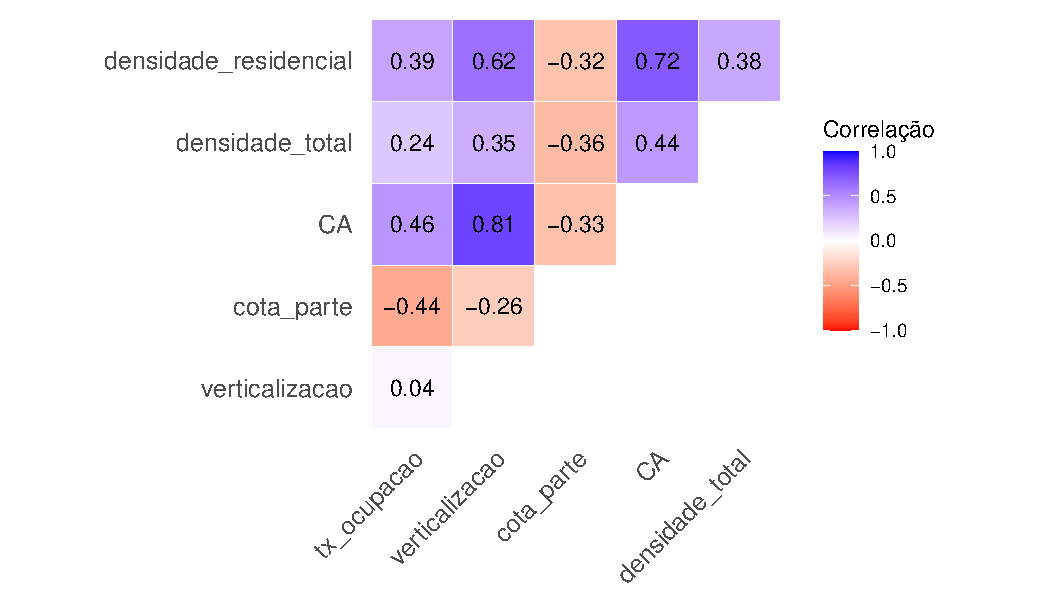
\includegraphics[width = .75\textwidth]{imagens/corrplot.pdf}
    \label{fig:corplot}
\end{figure}

Por fim, foi construída uma matriz de correlação (Figura \ref{fig:corplot}) entre as variáveis mais importantes. A correlação entre a densidade residencial e a total é de apenas 38\%, o que indica que de fato elas medem fenômenos diferentes. Os dois tipos de densidade apresentam a correlação na direção esperada com os indicadores apresentados, sendo que a residencial apresenta correlação mais forte. A alta correlação entre o CA e a verticalização é discutida no Apêndice \ref{appendix:verticalizacao}.

\section{Alguns resultados preliminares}
\label{sec:dados-res}

Apenas através da análise descritiva já é possível concluir que em boa parte da cidade os instrumentos regulatórios não funcionam, visto que as moradias não estão registradas nos sistemas públicos. Dessa forma, não importa qual regra for adotada pelo governo, estas áreas não serão impactadas por isso. Em termos numéricos, dos 4.996.529 domicílios registrados pelo Censo, há apenas 2.641.635 unidades habitacionais registradas no IPTU, o que representa um índice de moradia regular (em termos legais) de aproximadamente 52,87\%. Além disso, considerando uniforme o número de moradores por domicílio em cada setor censitário, estima-se que 5.944.595 de pessoas habitam em domicílios que não estão registrados no IPTU, o que representa 51,9\% da população de São Paulo. Outra descoberta relevante é de que grande parte das áreas mais densas da cidade estão em regiões de irregularidade. Isso é um indicativo de que há incentivos mais poderosos do que a regulação para definir a densidade de cada região.

Por fim, observa-se uma correlação positiva entre a densidade populacional, densidade construtiva e verticalização. Sobre a cota parte observada, há uma correlação negativa com a densiade populacional, visto que quanto mais unidades para uma dada área de terreno, menor a cota parte e maior a densidade populacional. Entretanto, apenas a correlação não é suficiente para determinar se os instrumentos são capazes de definir a densidade ou não. Na Seção \ref{sec:analise} será feita a análise com maior profundidade.


\chapter{Análise}
\label{sec:analise}

% Nessa seção, o objetivo é medir quantitativamente a capacidade dos padrões construtivos de definir a densidade populacional em uma determinada região através de modelos econométricos e de \textit{machine learning}.

\section{Densidade pela ótica da área de terreno residencial}
\label{sec:analiseR}

Para identificar como os padrões construtivos estão relacionados à densidade populacional residencial, foi elaborada uma regressão linear, especificada na equação a seguir. Uma maneira equivalente de representar a regressão está demonstrada na Equação \ref{eq:reg2}.


\begin{align}
    \textit{Densidade Populacional}_i =
    &\beta_0 + \beta_1 \cdot \textit{Densidade Construtiva}_i + & \rightarrow & \text{ CA}\nonumber\\
    &\beta_2 \cdot\textit{Cota Parte Observada}_i + & \rightarrow & \text{ Cota Parte} \\
    &\beta_3\cdot\textit{Verticalização}_i + \varepsilon_i & \rightarrow & \text{ Gabarito}\nonumber
    \label{eq:reg}
\end{align}
\begin{equation}
    \frac{\textit{População}_i}{\textit{A. Terreno}_i}=
    \beta_0+
    \beta_1\underbrace{\frac{\textit{A. Construída}_i}{\textit{A. Terreno}_i}}_\textit{CA}+
    \beta_2\underbrace{\frac{\textit{A. Terreno}_i}{\textit{N. unidades}_i}}_\textit{Cota Parte}+
    \beta_3\underbrace{\frac{\textit{A. Construída}_i}{\textit{A. Ocupada}_i}}_\textit{Verticalização}+\varepsilon_i
    \label{eq:reg2}
\end{equation}

Na análise conduzida, o nível da observação $i$ não pode ser o setor censitário, pois como discutido na Seção \ref{sec:dados}, o setor é construído de forma que um entrevistador sozinho consiga cobrí-lo por completo. Como consequência, áreas mais densas apresentarão setores censitários menores e, caso isso não seja controlado na regressão, haverá um grande problema de endogeneidade. Inclusive, na metodologia de separação dos setores censitários, há valores definidos de domicílios que cada setor censitário deve apresentar, de acordo com suas características \cite{IBGE2024}. Todavia, a área não pode ser um regressor, visto que haveria uma relação de simultaneidade: ao mesmo tempo que a área explica a densidade, a densidade também explica a área. Essa relação viola as suposições necessárias para interpretabilidade dos resultados.

Para contornar este problema, o nível da observação foi definido como cada célula do \textit{raster}, metodologia apresentada na Seção \ref{sec:dados}. Dessa forma, todas células apresentam o mesmo tamanho e este problema deixa de existir. Note que foram desconsideradas as células em que há dados do Censo, mas não há dados do IPTU, já que não se sabe os padrões construtivos nessas regiões. Em áreas em que há uma diferença muito grande entre número de domicílios registrados pelo Censo e unidades do IPTU, há menos confiança de que os indicadores calculados representam de fato a realidade. Portanto, em áreas em que o espectro de irregularidade está muito distante de 50\%, haverá viés nas estimações. Nesse sentido, foram feitas duas regressões, uma delas considera valores do espectro de irregularidade entre 35 e 65\% e a outra, entre 45 e 55\%. Como o corte escolhido para o espectro de irregularidade nas regressões não segue um critério objetivo, foi feita uma análise de sensibilidade dos resultados para variações desse critério arbitrário. Os resultados desse teste de robustez podem ser consultados no Apêndice \ref{appendix:robustez-corte}.

\begin{table}[h]
    \caption{Regressão para densidade populacional}
    \begingroup
\fontsize{10.5pt}{12.6pt}\selectfont
\begin{longtable}{lrlrlrlrl}
\toprule
 & \multicolumn{4}{c}{Todos os setores} & \multicolumn{3}{c}{Espectro irregularidade: 40 a 60\%} &  \\ 
\cmidrule(lr){2-5} \cmidrule(lr){6-8}
 & \multicolumn{2}{c}{Nível (A)    } & \multicolumn{2}{c}{Log (B)    } & \multicolumn{2}{c}{Nível (C)    } & \multicolumn{2}{c}{Log (D)    } \\ 
\cmidrule(lr){2-3} \cmidrule(lr){4-5} \cmidrule(lr){6-7} \cmidrule(lr){8-9}
  & Coeficiente & * & Coeficiente  & *  & Coeficiente   & *   & Coeficiente    & *    \\ 
\midrule\addlinespace[2.5pt]
(Intercept) & 11046.375 & *** & 8.987 & *** & 8632.310 & *** & 9.109 & *** \\ 
cota\_parte & -0.004 &  & 0.000 & *** & -6.973 & *** & -0.002 & *** \\ 
verticalizacao & -249.059 &  & -0.075 & ** & -48.242 &  & -0.026 &  \\ 
CA & 1211.554 & *** & 0.243 & *** & 1672.931 & *** & 0.143 & *** \\ 
{R2} & {0.022} & {} & {0.052} & {} & {0.249} & {} & {0.328} & {} \\ 
R2 ajustado & 0.020 &  & 0.050 &  & 0.245 &  & 0.325 &  \\ 
Observações & 1255 &  & 1254 &  & 553 &  & 553 &  \\ 
\bottomrule
\end{longtable}
\endgroup


    \label{tab:reg}
    \addtocounter{table}{-1}
\end{table}

O primeiro resultado interessante de ser analisado é como não são fortes as evidências de que a verticalização influencia a densidade. Do ponto de vista teórico isso faz sentido, visto que com o CA mantido constante, há um \textit{trade-off} direto entre verticalização e área ocupada. Dessa forma, essa escolha torna-se principalmente estética, dado que a área construída se mantém igual. Ao analisar a regressão (D), com a densidade em log, pode-se inferir que ao diminuir em um metro quadrado a cota parte observada, espera-se que com os outros componentes constantes, a densidade populacional aumente em média 0,2\%. O aumento de 1 na densidade construtiva, segundo os resultados da regressão (D), tem como consequência um aumento esperado médio na densidade populacional de 27,4\%, caso os outros componentes se mantenham iguais. O intercepto não apresenta interpretação\footnote{Na prática é impossível que uma área tenha cota parte igual a zero, já que é calculada pela área do terreno sobre o número de unidades, então apresenta o valor máximo igual a área do terreno e se aproxima de zero na medida em que o número de unidades é infinito.}.

Todavia, há dois pontos que devem ser levantados. Primeiramente, partindo da hipótese de que os padrões construtivos apresentados não são capazes de definir a densidade, os parâmetros da regressão estarão contaminados pelo viés advindo da omissão de regressores relevantes. Em segundo lugar, a forma funcional apresentada na Equação \ref{eq:reg2} não foi especificada com base em alguma teoria econômica ou algum tipo de embasamento, o que implica que há boas chances de ela estar inadequada.

Nesse sentido, foi tomada uma abordagem diferente, na qual foi construída uma \textit{random forest} \cite{wright2015ranger}. A vantagem dessa abordagem é que não é necessário especificar uma forma funcional, já que a própria metodologia seleciona as variáveis mais importantes e constrói uma regressão não linear. No exemplo de árvore de regressão apresentado na Figura \ref{fig:tree}, cada círculo representa um nó de decisão, então no primeiro à esquerda, por exemplo, é testado se a cota parte é menor ou maior que 472 metros quadrados. A depender do resultado, a observação é direcionada para o próximo nó de decisão até que chegue na folha (na figura, a folha está representada pelo quadrado à direita). É interessante notar que as folhas cuja predição apresenta a maior densidade são as com cota parte pequena e CA alto. No procedimento de criação da \textit{random forest}, foram feitas 100 mil árvores de regressão como a apresentada na figura, cada uma com diferentes nós de decisão. 

\begin{figure}[h]
    \centering
    \caption{Exemplo de uma das árvores de regressão}
    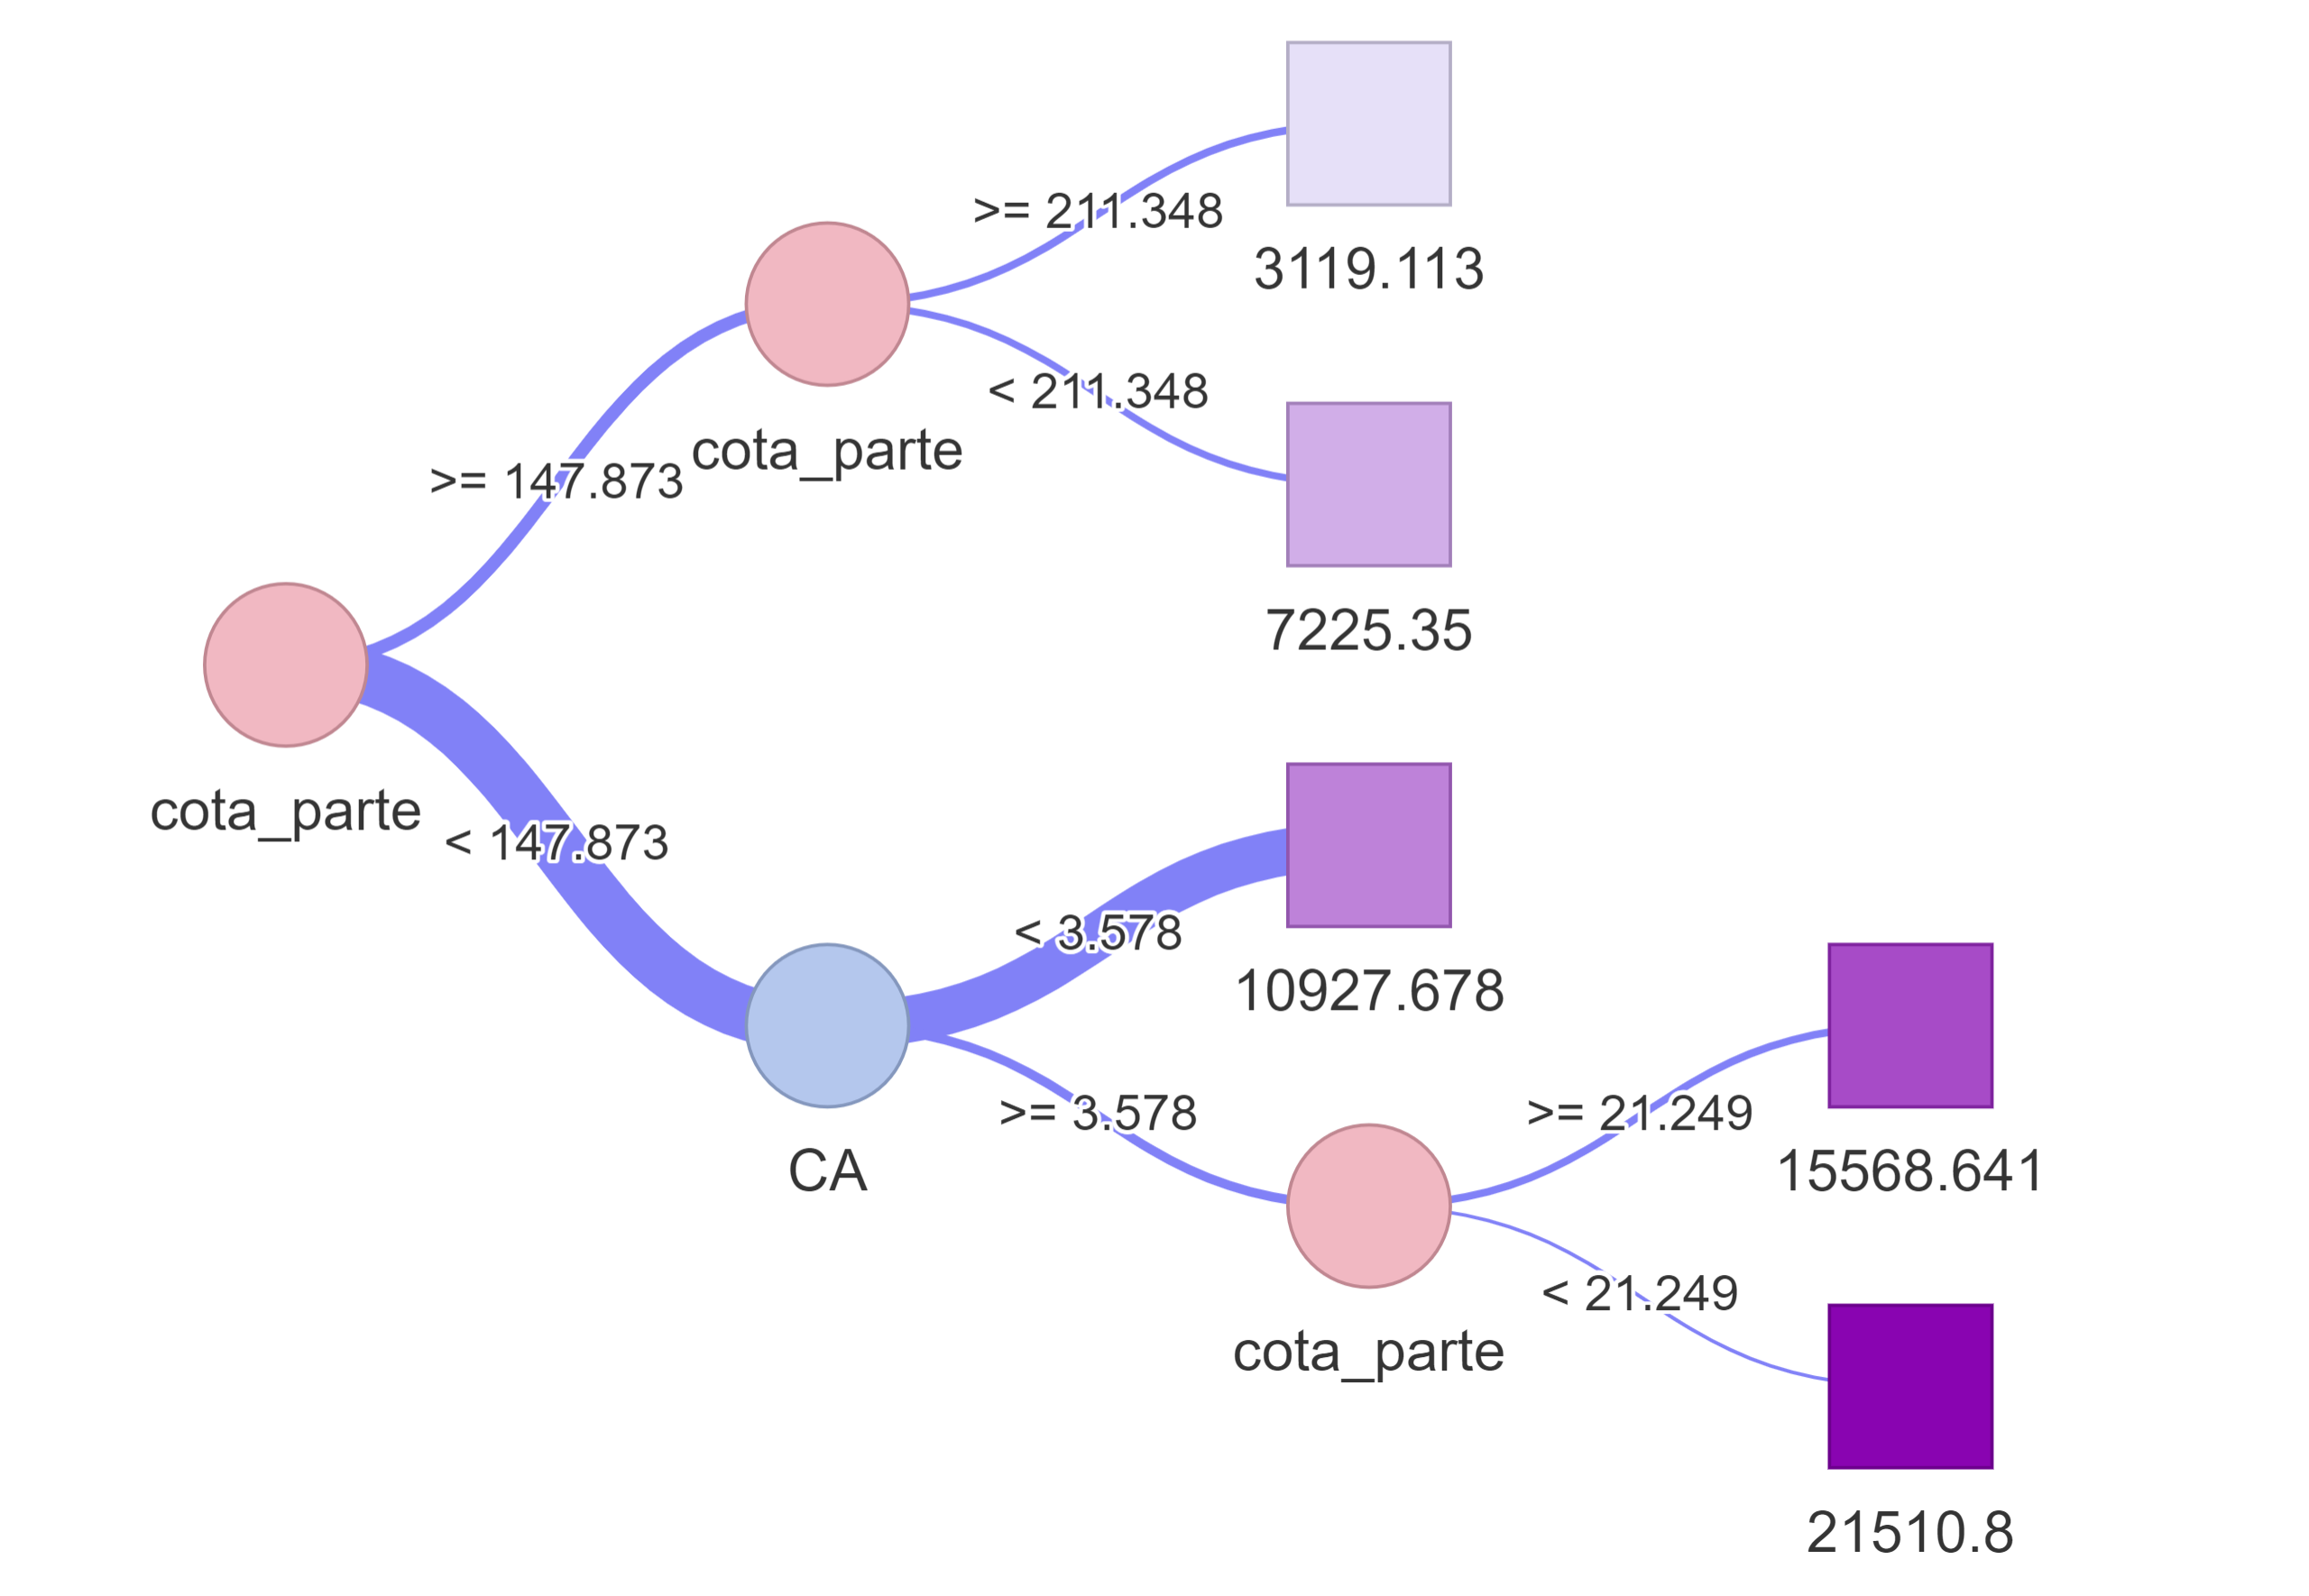
\includegraphics[width = \linewidth]{imagens/tree_example.png}
    \label{fig:tree}
\end{figure}

Para construir o modelo de floresta de regressão, é necessário dividir a base de dados em treino e teste, de forma que não haja \textit{overfit}, ou seja, o modelo não ``decora'' os dados. As árvores foram construídas a partir das células que apresentam o espectro de irregularidade entre 40 e 60\%. Com o objetivo de tornar a comparação justa, foi refeita a equação de regressão linear, como especificado na Tabela \ref{tab:reg} (C), mas apenas com os dados de treino iguais à floresta. Depois, tanto a floresta de regressão, quanto a regressão linear previram os mesmos dados de teste, para comparar os modelos. O $R^2$ na base de teste para o modelo de regressão linear foi de 50,6\%, enquanto da floresta de regressão foi de 81,9\%. Apesar da regressão apresentar um bom coeficiente de explicação, o maior sucesso da árvore de regressão é uma evidência de que a relação entre as variáveis apresentadas não é exatamente o que foi especificado na Equação \ref{eq:reg2}.

Para analisar quais informações do modelo são mais importantes, é possível realizar um procedimento de permutação no qual é introduzido ruído nos regressores para testar como isso afeta o erro do modelo \cite{breiman2001random, Nembrini2018}. Esse processo de permutação permite quantificar a importância de cada regressor para explicar a variável dependente. Na Figura \ref{fig:importancia-restrito} é possível observar os resultados. A característica construtiva mais relevante para definir a densidade populacional foi a cota parte observada, seguida pela densidade construtiva e por fim a verticalização.

\begin{figure}[h]
    \centering
    \caption{Importância do padrão construtivo para explicar a densidade, para espectro entre 40 e 60\%}
    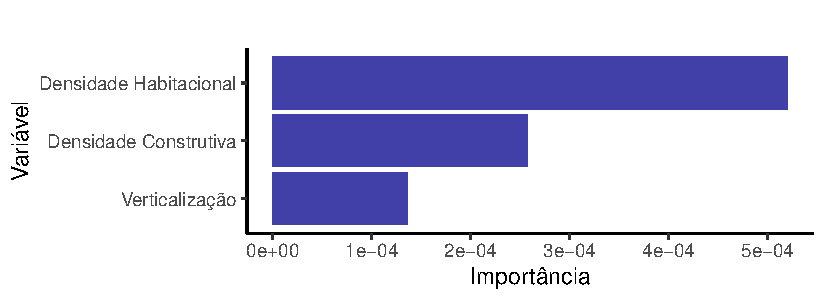
\includegraphics[width = .8\linewidth]{imagens/var_importance_restrito.pdf}
    \label{fig:importancia-restrito}
\end{figure}

Depois, foi fornecido à floresta de regressão mais informações que estão disponíveis na base de dados do IPTU, para avaliar se há algum outro componente importante para definir a densidade populacional. Como resultado, o novo $R^2$ passou a ser de 84,7\%, o que representa um ganho de 2,8$p.p.$ Isso é um indicativo de que as outras variáveis não trazem muitas novas informações para prever a densidade populacioal da região. Entre as novas variáveis do modelo, estão o número total de unidades e as áreas do terreno, construída e ocupada. Na Figura \ref{fig:importancia} está disposto o resultado do procedimento quando são incluídas outras variáveis disponíveis na \textit{random forest}. É notável que a área do terreno apresenta uma importância significativa na definição da densidade residencial. Um motivo que pode contribuir para isso é, como apontado na Equação \ref{eq:reg2}, que a área do terreno é utilizada no cálculo da densidade.

\begin{figure}[h]
    \centering
    \caption{Importância das variáveis do modelo para explicar a densidade, para espectro entre 40 e 60\%}
    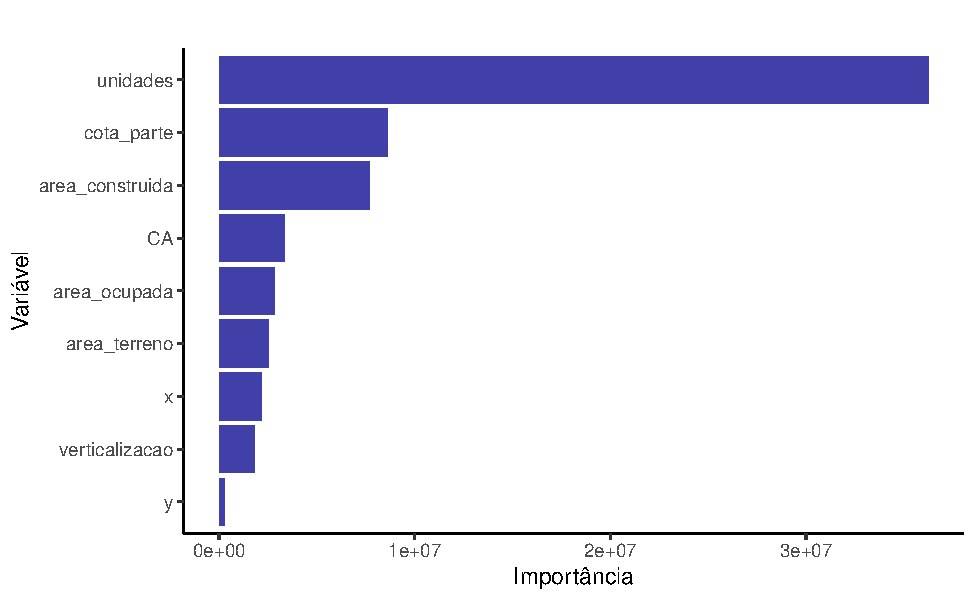
\includegraphics[width = .95\linewidth]{imagens/var_importance.pdf}
    \label{fig:importancia}
\end{figure}

\section{Densidade pela ótica da área total}

Os resultados apresentados até então foram relativos à densidade residencial, que é diferente da densidade total, como desenvolvido na Seção \ref{sec:dados}. Caso o objetivo dos instrumentos seja regulamentar um novo lote residencial a ser construído, utilizar a ótica da área do terreno é o que mais faz sentido. Todavia, caso a intenção do governo seja de regulamentar uma região como um todo, não importando o uso de solo, faz mais sentido considerar a densidade como uma fração da área total. Isso implica considerar terrenos residenciais e não residenciais no cômputo da densidade, como áreas públicas, comerciais, de lazer, etc. Uma área com um grande parque, por exemplo, na ótica da área de terreno (densidade residencial), não é responsável por reduzir a densidade em uma região, e dessa forma os instrumentos não serão capazes de compensar a densidade perdida por outros usos do solo. 

A cota parte, que define o número mínimo de unidades que o lote deve apresentar, não considera quanto da área na região é alocada para outros tipos de uso de solo. Nesse sentido, considerando o exemplo do parque, um novo empreendimento não deve apresentar mais unidades por estar ao lado de uma área com amenidades e menor área de terreno residencial. Para validar se esta hipótese é verdadeira, foi realizado o mesmo procedimento utilizado para a densidade residencial, mas agora regredindo a densidade na ótica da área total. A importância de cada variável pode ser observada na Figura \ref{fig:importancia_densmod}.

\begin{figure}[h]
    \centering
    \caption{Importância das variáveis, mas com a densidade calculada através da população sobre a área total. Espectro de irregularidade entre 40 e 60\%}
    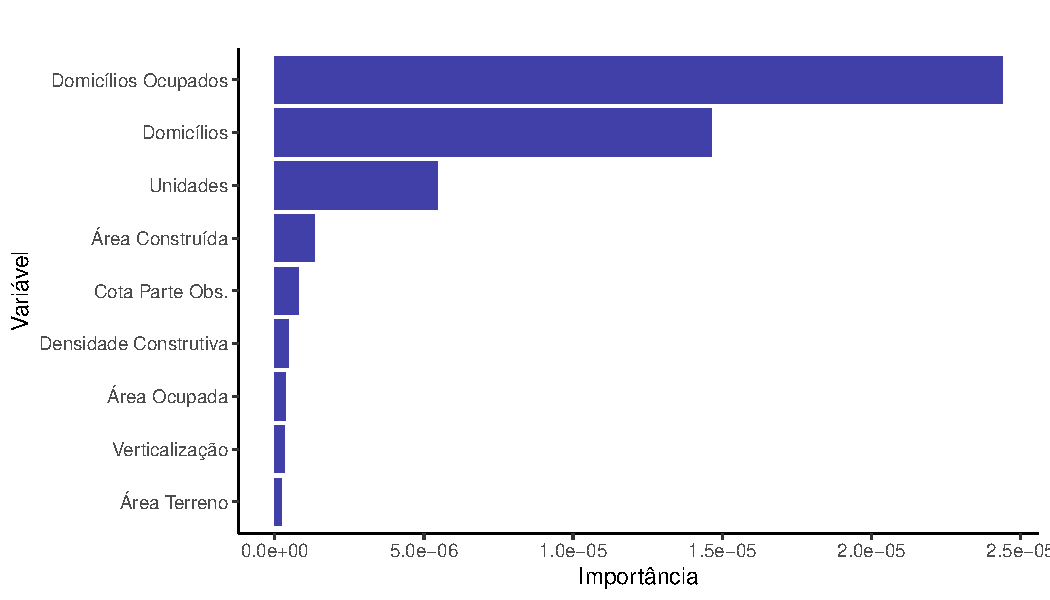
\includegraphics[width = .95\linewidth]{imagens/var_importance_densmod.pdf}
    \label{fig:importancia_densmod}
\end{figure}

É interessante perceber que a ferramenta que se demonstra mais importante para definir a densidade total é o número de domicílios, especialmente os ocupados. Isso é um forte indicativo de que os instrumentos, apesar de serem capazes de definir a densidade de uma área de terreno, não apresentam a mesma eficácia para definir a densidade de uma região. O modelo de regressão linear, como especificado na Equação \ref{eq:reg2}, mas regredindo a densidade total ao invés da residencial, apresenta um $R^2$ na base de teste de apenas 28,1\%, o que representa uma queda no poder de explicação. Com as mesmas variáveis explicativas, a árvore de regressão atinge um $R^2$ de 44,2\%. Agora, ao introduzir-se as outras variáveis disponíveis, as que estão demonstradas na Figura \ref{fig:importancia_densmod}, o $R^2$ na base de treino passa a ser de 96,1\%, mais que duas vezes maior do que o modelo restrito apenas com as três variáveis. 

\section{Densidade prevista para determinados padrões construtivos}

Com base na \textit{random forest} construída na Seção \ref{sec:analiseR}, é possível estimar a população de um determinado lote, com base em seus padrões construtivos. Para fins ilustrativos, foi considerado um lote cuja área é de 5.000$m^2$\footnote{como referência, esta é aproximadamente a área do lote do MASP}. Nesse lote hipotético, a depender do CA, cota parte e verticalização observados, pode-se estimar a população que o habitaria. Na Figura \ref{fig:previsoes} é possível analisar os resultados.

\begin{figure}[h]
    \centering
    \caption{Previsões de população para cada padrão construtivo, considerando um terreno de 5.000$m^2$}
    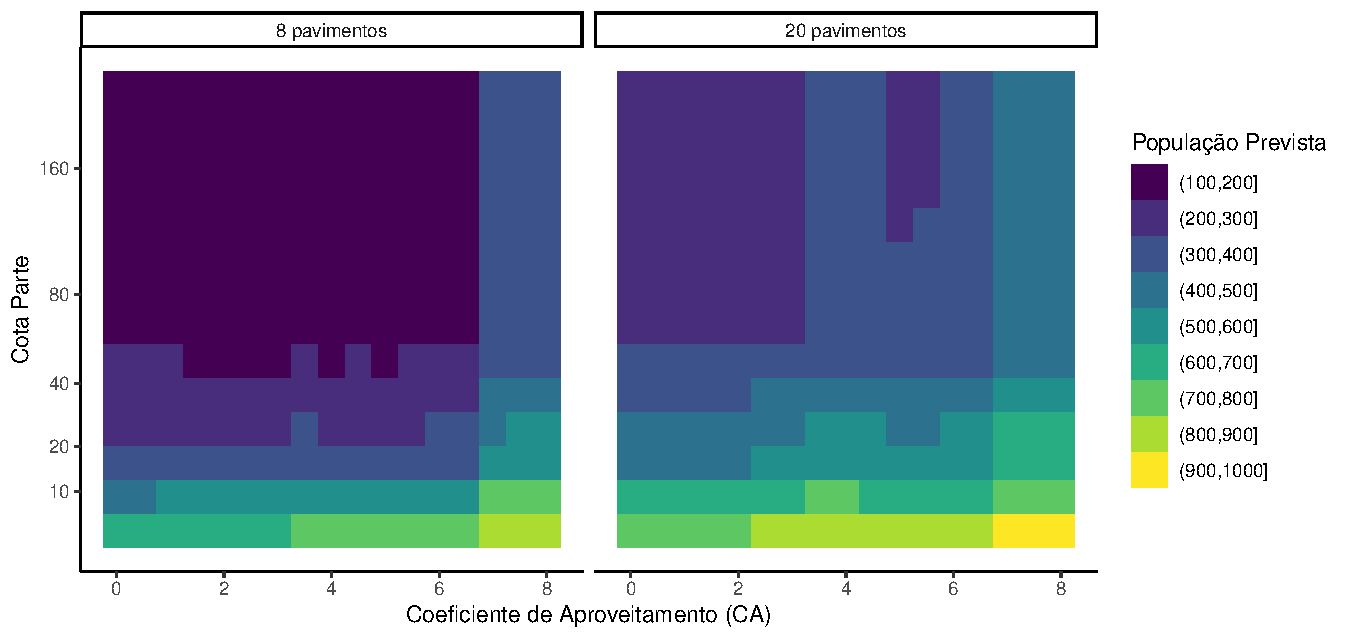
\includegraphics[width = \textwidth]{imagens/previsoes.pdf}
    \label{fig:previsoes}
\end{figure}

Em linha com os resultados apresentados da regressão linear, na medida em que se aumenta o CA e se desloca no eixo $x$, a estimativa da densidade populacional aumenta. Ainda, a alteração na cota parte (deslocamento no eixo $y$) causa um impacto maior na estimativa da população. A modificação de 8 para 20 pavimentos apresenta mudanças na população, mas em magnitude menos relevante.


\chapter{Conclusão}
\label{sec:conclusao}

As evidências apontam que dada um determinada área de terreno, os padrões construtivos observados são capazes de definir a densidade populacional com pequena margem para outros componentes mudarem o resultado. Isso significa que caso o governo tenha o objetivo de definir a densidade populacional exata de um lote, se impuser seu coeficiente de aproveitamento (CA), cota parte e número de pavimentos, provavemente alcançará seus objetivos. Como observado na Figura \ref{fig:previsoes}, por exemplo, em um lote de 5.000$m^2$, caso ordene a construção de um empreendimento de 20 pavimentos, com um CA de 4 e uma cota parte de 20, é esperado que aproximadamente 560 pessoas o habitem. 

Entre as características construtivas que se demonstraram mais relevantes para definir a densidade populacional, a densidade habitacional, calculada pela cota parte, foi a que mais se destacou. Este resultado é muito relevante, visto que a regulação sobre a cota parte existe no PDE apenas em regiões de eixos de estruturação da transformação urbana (EETUs), nos quais a cota parte mínima é de 20$m^2$. A densidade construtiva, medida pelo coeficiente de aproveitamento (CA) também apresentou grande relevância para definir a densidade. Já sobre a verticalização, houve evidências fracas que apontassem para sua importância. Como explicado no Apêndice \ref{appendix:verticalizacao}, quando o nível de CA é definido, a verticalização passa a ser uma consequência direta da taxa de ocupação do terreno, e vise versa. Nesse sentido, faz sentido que mudanças no gabarito, caso o CA se mantenha igual, tragam pouco impacto na densidade.

Dessa forma, para o bem ou para o mal, caso a prefeitura consiga regulamentar os padrões construtivos, será capaz de definir a densidade em cada parte da cidade. Como pontuado na Seção \ref{sec:intro-regulacao}, este poder não vem desacompanhado de perigos, caso seja mal administrado. Uma agenda de pesquisa que se mostra importante à luz dos resultados trazidos nessa pesquisa, refere-se ao estado da oferta e demanda por habitação em São Paulo. Caso a demanda nas regiões centrais esteja sendo reprimida pela regulação, é possível que ela esteja causando um espraiamento urbano, resultado que o próprio plano diretor almeja combater.

Por fim, como apontado na Seção \ref{sec:dados-res}, cerca de metade das moradias da cidade se encontra em situação de informalidade e, portanto, a regulação não surte efeito direto nelas. Para fins de planejamento urbano, este é um problema grave e suas raízes devem ser investigadas. Uma hipótese que está em linha com os pontos trazidos anteriormente, se refere à possibilidade da demanda reprimida e preços elevados gerarem incentivos para a formação de um mercado de moradia informal.


% Responder categoricamente que os instrumentos são eficientes seria um forte reducionismo, visto que eficiência é um espectro largo e relativamente arbitrário. Ainda assim, os testes de hipótese apresentados ao longo da Seção \ref{sec:analise} apontam que o CA e a cota parte são importantes para definir a densidade populacional de uma região, enquanto a verticalização não. Ainda, foi quantificado que a cota parte apresenta uma maior importância, ao comparada com o CA.

% Todavia, também foi discutido como outros fatores que não foram medidos podem impactar a densidade. A teoria econômica indica que a proximidade à oferta de emprego é um fator central na fisiologia da cidade, por exemplo. No entanto este fator não é considerado no cálculo do CA ou cota parte permitida em cada região e, portanto, não foi considerada nessa análise. Como uma futura agenda de pesquisa é importante investigar estes outros fatores e como eles se comparam com a eficiência dos atuais instrumentos na determinação da densidade.

% Outra descoberta relevante foi sobre a gravidade da miopia que a prefeitura apresenta sobre a moradia na cidade, haja vista os milhões de domicílios que não estão inscritos no Cadastro Imobiliário Fiscal, e, portanto, não pagam imposto e não necessariamente seguem as regulamentações impostas para garantir o cumprimento dos objetivos da cidade. Em termos numéricos, foi estimado que aproximadamente 53\% dos domicílios estão cadastrado, enquanto todos os outros estão por fora dos sistemas públicos.

% Nesse sentido, mesmo que os instrumentos sejam os mais eficientes possíveis, eles podem impactar no máximo metade da cidade, enquanto a outra metade é regida por instituições informais. Entretanto, é importante destacar que observa-se nessas regiões de moradia informal um adensamento muitas vezes maior do que em regiões regulares. A região mais densa da cidade é a favela de Paraisópolis, o que indica que há forças de adensamento mais fortes que a regulação.